\chapter{Introduction to data}
\label{introductionToData}

%\begin{tipBox}{\tipBoxTitle[Chapter Goal:]{Thinking about data}
%Understand basics about data organization, data types, numerical summaries of data, graphical summaries of data, and foundational techniques for data collection. We begin and end the chapter with case studies.}
%\end{tipBox}

Scientists seek to answer questions using rigorous methods and careful observations. These observations -- collected from the likes of field notes, surveys, and experiments -- form the backbone of a statistical investigation and are called \term{data}. Statistics is the study of how best to collect, analyze, and draw conclusions from data. It is helpful to put statistics in the context of a general process of investigation:
\begin{enumerate}
\setlength{\itemsep}{0mm}
\item Identify a question or problem.
\item Collect relevant data on the topic.
\item Analyze the data.
\item Form a conclusion.
%\item Make decisions based on the conclusion.
\end{enumerate}
Statistics as a subject focuses on making stages (2)-(4) objective, rigorous, and efficient. That is, statistics has three primary components: How best can we collect data? How should it be analyzed? And what can we infer from the analysis?

The topics scientists investigate are as diverse as the questions they ask. However, many of these investigations can be addressed with a small number of data collection techniques, analytic tools, and fundamental concepts in statistical inference. This chapter provides a glimpse into these and other themes we will encounter throughout the rest of the book. We introduce the basic principles of each branch and learn some tools along the way. We will encounter applications from other fields, some of which are not typically associated with science but nonetheless can benefit from statistical study.

\section[Case study]{Case study: treating heart attack patients with a new drug}
\label{basicExampleOfSulphinpyrazone}

%We first consider a scientific study to introduce basic ideas about data collection, summary, and conclusions. While we encourage the reader to think about each of the bolded terms, we will revisit all terms in greater detail later this chapter.

Section~\ref{basicExampleOfSulphinpyrazone} introduces a classic challenge in statistics: evaluating the efficacy of a pharmaceutical treatment. Terms in this section, and indeed much of this chapter, will all be revisited later in the text, and in greater detail. The plan for now is simply to begin getting a sense of the role statistics can play in practice.

In this first section, we consider an experiment used to evaluate whether a drug, sulphinpyrazone, reduces the risk of death in heart attack patients\footnote{Anturane Reinfarction Trial Research Group. 1980. Sulfinpyrazone in the prevention of sudden death after myocardial infarction. New England Journal of Medicine 302(5):250-256.}. In this study, we might start by writing the principle question we hope to answer:
\begin{quote}
Does administering sulphinpyrazone to a heart attack patient reduce the risk of death?
\end{quote}

The researchers who asked this question collected data on 1,475 heart attack patients. 
%To answer this question, researchers %who asked it %proceeded to the second stage of the investigative process: data collection. They 
%collected data on 1475 heart attack patients who volunteered for their study. 
Each volunteer patient was randomly assigned to one of two groups:
\begin{itemize}
\item[]\termsub{Treatment group}{treatment group}. Patients in the treatment group received the experimental drug, sulphinpyrazone.
\item[]\termsub{Control group}{control group}. Patients in the control group did not receive the drug but instead were given a \term{placebo}, which is a fake treatment with no chemical agents that is made to look real.
\end{itemize}
In the end, there were 733 patients in the treatment group and 742 patients in the control group. The patients were not told which group they were in, and the reason for this secrecy is that patients who know they are being treated often times show improvement (or slower degeneration) regardless of whether the treatment actually works. This improvement is called a \term{placebo effect}. If patients in the control group were not given a placebo, we would be unable to sort out whether any observed improvement was due to the placebo effect or the treatment's effectiveness.

After 24 months in the study, each patient was either still alive or had died; this information describes the patient's \term{outcome}. So far, there are two relevant characteristics about each patient: patient \var{group} and patient \var{outcome}. We could organize these data into a table. One common organization method is shown in Table~\ref{sulphinpyrazoneDF}, in which each patient is represented by a row, and the columns relate to the information known about the patients.
\begin{table}[h]
\centering
\begin{tabular}{l cc}
\hline
Patient	&	\var{group}	&	\var{outcome} \\
\hline
1		&	\resp{treatment} &	\resp{lived} \\
2		&	\resp{treatment} &	\resp{lived} \\
$\vdots$	&	$\vdots$	  &	$\vdots$ \\
1475	&	\resp{control} &	\resp{lived} \\
\hline
\end{tabular}
\caption{Three patients from the sulphinpyrazone study.}
\label{sulphinpyrazoneDF}
% trmt <- c(rep('drug', 733), rep('placebo', 742))
% outcome <- c(rep(c('lived', 'died'), c(692, 41)), rep(c('died', 'lived'), c(60, 682)))
\end{table}

Considering data from each patient individually would be a long, cumbersome path towards answering the original research question. Instead, it is often more useful to perform a data analysis, considering all of the data at once. We first might summarize the raw data in a more helpful way, like that shown in Table~\ref{sulphinpyrazoneResultsInIntro}. In this table, we can quickly see what happened over the entire study. For instance, to identify the number of patients in the treatment group who died, we could look at the intersection of the \resp{treatment} row and the \resp{died} column: 41.
\begin{table}[h]
\centering
\begin{tabular}{l l cc rr}
& & \multicolumn{2}{c}{\var{outcome}} \\
  \cline{3-4}
		&			& 	\resp{lived} 	& \resp{died} & Total & \hspace{3mm}  \\ 
  \cline{2-5}
		&	\resp{treatment} 	& 692    		& 41   & 733  	 \\ 
  \raisebox{1.5ex}[0pt]{\var{group}}		&	\resp{control} 	& 682    		& 60     & 742	 \\ 
  \cline{2-5}
  		&	Total		& 1374	& 101	&  1475 \\
  \cline{2-5}
\end{tabular}
\caption{Descriptive statistics for the sulphinpyrazone study.}
\label{sulphinpyrazoneResultsInIntro}
\end{table}

\begin{exercise}
Of the 733 patients in the treatment group, 41 died. Using these two numbers, compute the proportion of patients who died in the treatment group. Answer in the footnote\footnote{The proportion of the 733 patients who died is $41/733 = 0.056$.}.
\end{exercise}

We can compute summary statistics from the summary table. A \term{summary statistic} is a single number summarizing a large amount of data\footnote{Formally, a summary statistic is a value computed from the data. Some summary statistics are more useful than others.}. For instance, the primary results of the study could be placed in two summary statistics: the proportion of people who died in each group.
\begin{itemize}
\setlength{\itemsep}{0mm}
\item[] Proportion who died in the treatment group: $41/733 = 0.056$.
\item[] Proportion who died in the control group: $60/742 = 0.081$.
\end{itemize}
These two summary statistics are useful in evaluating whether the drug worked. There is an observed difference in the outcomes: the death rate was 2.5\% lower in the treatment group. We will encounter many more summary statistics throughout this first chapter.

Here we now move into the fourth stage of the investigative process: drawing a conclusion. We might ask, does this 2.5\% difference in death rates provide convincing evidence that the drug worked? Even if the drug didn't work, we wouldn't necessarily observe the exact same death rate in the two groups. Maybe the difference of 2.5\% was just due to chance. Regrettably, our analysis does not indicate whether what we are seeing is real or a random fluctuation. We will have to wait until a later section before we can make a more formal assessment.

We conduct a more formal analysis in Section~\ref{caseStudyOfSulphinpyrazone} (optional) for this drug study so that we can draw a more careful conclusion from the data. However, this analysis will not make much sense before we discuss additional principles, ideas, and tools of statistics in Sections~\ref{dataBasics}-\ref{experimentsSection}. % In order to discuss some basic reasons behind different data collection techniques, we discuss this topic close to the end of this chapter.

\section{Data basics}
\label{dataBasics}

Effective presentation and description of data is a first step in most analyses. This section introduces one structure for organizing data as well as data terminology that will be used throughout this book.

\subsection{Observations, variables, and cars}

Table~\ref{carsDF} displays rows 1, 2, and 54 of a data set concerning cars from 1993. These observations (measurements) of 54 cars will be referred to as the \data{cars} data set\footnote{Lock RH. 1993. 1993 New Car Data. Journal of Statistics Education 1(1).}.

Each row in the table represents a single car or \term{case}\footnote{A case may also be called a \term{unit of observation} or an \term{observational unit}.} and contains six characteristics or measurements for that car. For example, car 54 is a midsize car that can hold 5 people.

Each column of Table~\ref{carsDF} represents an attribute known about each case, and these attributes are called \term{variables}. For instance, the \var{mpgCity} variable holds the city miles per gallon rating of every car in the data set.

In practice, it is especially important to ask clarifying questions to ensure important aspects of the data are understood. For instance, it is always important to be sure we know what each variable means and the units of measurement. Descriptions of all six {car} variables are given in Table~\ref{carsVariables}.


\subsection{Data Matrices}

\begin{table}[t]
\centering
\begin{tabular}{c ccc ccc}
  \hline
 & \var{type} & \var{price} & \var{mpgCity} & \var{drivetrain} & \var{passengers} & \var{weight} \\
  \hline
1 & small & 15.9 & 25 & front &  5 & 2705 \\
  2 & midsize & 33.9 & 18 & front &  5 & 3560 \\
%  3 & midsize & 37.7 & 19 & front &  6 & 3405 \\
$\vdots$ & $\vdots$ & $\vdots$ & $\vdots$ & $\vdots$ & $\vdots$ & $\vdots$ \\
  54 & midsize & 26.7 & 20 & front &  5 & 3245 \\
  \hline
\end{tabular}
\caption{Three rows from the \data{cars} data matrix.}
\label{carsDF}
\end{table}

\begin{table}[t]
\centering\small
\begin{tabular}{lp{9.5cm}}
\hline
{\bf variable} & {\bf description} \\
\hline
%\begin{itemize}
\var{type} & car type (\resp{small}, \resp{midsize}, or \resp{large}) \\
\var{price} & the average purchase price of the vehicles in \$1000's (positive number) \\
\var{mpgCity} & rated city mileage in miles per gallon (positive number) \\
\var{drivetrain} & the drivetrain, also called the powertrain (\resp{front}, \resp{rear}, \resp{4WD}) \\
\var{passengers} & passenger capacity (positive whole number, taking values \resp{4}, \resp{5}, or \resp{6}) \\
\var{weight} & car weight in pounds (positive number) \\
%\end{itemize}
\hline
\end{tabular}
\caption{Variables and their descriptions for the \data{cars} data set.}
\label{carsVariables}
\end{table}

The data in Table~\ref{carsDF} represent a \term{data matrix}, which is a common way to organize data. Each row of a data matrix corresponds to a separate case, and each column corresponds to a variable. A data matrix for the drug study introduced in Section~\ref{basicExampleOfSulphinpyrazone} is shown in Table~\ref{sulphinpyrazoneDF} on page~\pageref{sulphinpyrazoneDF}, where patients were the cases and there were two recorded variables.

Data matrices are convenient for recording data as well as analyzing data using a computer. In data collection, if another individual or case is added to the data set, an additional row can be easily added. Similarly, additional columns can be added for new variables.

\begin{exercise}
Researchers collected body measurements for bushtail possums in Eastern Australia\footnote{Lindenmayer DB, Viggers KL, Cunningham RB, and Donnelly CF. 1995. Morphological variation among columns of the mountain brushtail possum, Trichosurus caninus Ogilby (Phalangeridae: Marsupiala). Australian Journal of Zoology 43:449-458.}. They trapped 104 possums and recorded age, gender, head length, and four other pieces of information for each possum. How might these data be organized in a data matrix? Answer in the footnote\footnote{Here each possum represents a case, and there are seven pieces of information recorded for each case. A table with 104 rows and seven columns could hold these data, where each row represents a possum and each column represents a particular type of measurement or recording.}.
\end{exercise}

\subsection{Types of variables}
\label{variableTypes}

Examine the \var{type}, \var{price}, \var{drivetrain}, and \var{passengers} variables in the \data{cars} data set. Each of these variables is inherently different from the other three yet many of them share certain characteristics.

%First consider \var{price}, which is said to be a \term{numerical} variable since it can take a wide range of numerical values and those numbers have a meaningful ordering. That is, all 54 cars could be ordered according to \var{price}, and this ordering would have meaning (e.g. least expensive to most expensive). On the other hand, telephone area codes generally are not numerical since no clear meaning is derived from ordering the area codes.

First consider \var{price}, which is said to be a \term{numerical} variable since it can take a wide range of numerical values, and it is sensible to add, subtract, or take averages with those values. On the other hand, we do not classify a variable reporting telephone area codes as numerical since their average, sum, and difference have no clear meaning.

The \var{passengers} variable is also numerical, although it seems to be a little different than \var{price}. The variable \var{passengers} can only take whole positive numbers (\resp{1}, \resp{2}, ...) since it is not possible to have 4.5 passengers. The variable \var{passengers} is said to be \term{discrete} since it only can take numerical values with jumps (e.g. 3 or 4, but not any number in between). On the other hand, \var{price} is said to be \term{continuous}.

The variable \var{drivetrain} can only take a few different values: \resp{front}, \resp{rear}, and \resp{4WD}. Because the responses themselves are categories, \var{drivetrain} is called a \term{categorical} variable\footnote{Sometimes also called a \term{nominal} variable.}. The three possible values (\resp{front}, \resp{rear}, \resp{4WD}) are called the variable's \term{levels}.

\begin{figure}
\centering
\includegraphics[width=0.48\textwidth]{01/figures/variables/variables}
\caption{Breakdown of variables into their respective types.}
\label{variables}
\end{figure}

Finally, consider the \var{type} variable describing whether a car is \resp{small}, \resp{medium}, or \resp{large}. This variable seems to be a hybrid: it is a categorical variable but the levels have some inherent ordering. A variable with these properties is called an \term{ordinal} variable. To simplify analyses, any ordinal variables in this book will be treated as categorical variables.


\begin{example}{Data were collected about students in a statistics course. Three variables were recorded for each student: number of siblings, student height, and whether the student had previously taken a statistics course. Classify each of the variables as continuous numerical, discrete numerical, or categorical.}
The number of siblings and student height represent numerical variables. Because the number of siblings is a count, it is discrete. Height varies continuously, so it is a continuous numerical variable. The last variable classifies students into two categories -- those who have and those who have not taken a statistics course -- which makes this variable categorical.
\end{example}

\begin{exercise}
In the sulphinpyrazone study from Section~\ref{basicExampleOfSulphinpyrazone}, there were two variables: \var{group} and \var{outcome}. Are these numerical or categorical variables?
\end{exercise}

%\begin{example}{What are the variable types of \var{sex} and \var{headL} in the \data{possum} data set?}
%Because the \var{sex} variable takes non-numerical values, it is a categorical variable. Because \var{headL} has numbers as a response and it is meaningful to order these observations by their numbers, it is a numerical variable. More specifically, since \var{headL} can be any length, this variable is a \emph{continuous} numerical variable even though the measured values are all rounded to one decimal.
%\end{example}

%\begin{exercise}
%Identify each of the remaining variables in the \data{possum} data set as either continuous numerical, discrete numerical, or categorical.
%\end{exercise}

%\begin{exercise}\label{possumSiteExer}
%An additional variable was recorded for the \data{possum} data set called \var{site}. Each possum's site is represented a number \resp{1}, \resp{2}, ..., or \resp{7}, however, the ordering of the numbers doesn't actually hold meaning. Is this a numerical or categorical variable? Answer in the footnote\footnote{Because the order of the numbers holds no meaning, this is a categorical variable.}.
%\end{exercise}

\subsection{Relationships among variables}
\label{variableRelations}

\setlength{\captionwidth}{99mm}
\begin{figure}
\begin{center}
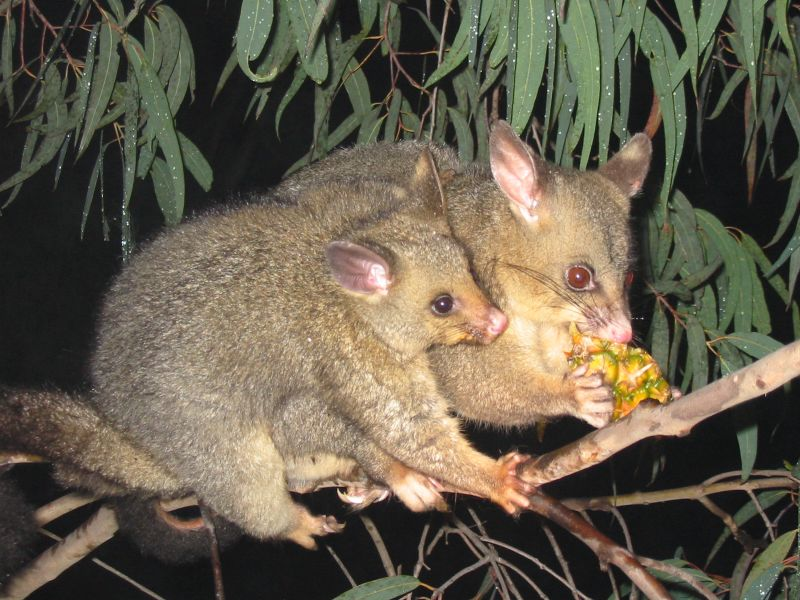
\includegraphics[width=95mm]{01/figures/possumPic/possumPic.jpg} \\
\addvspace{2mm}
\begin{minipage}{\textwidth}
   \caption[possums]{The common brushtail possum of Australia.\vspace{-1mm} \\
   -----------------------------\vspace{-2mm}\\
   {\footnotesize Photo by wollombi on Flickr: \urlwofont{http://flickr.com/photos/wollombi/58499575/}}\vspace{-8mm}}
   \label{possumPic}
\end{minipage}
\vspace{3mm}
\end{center}
\end{figure}
\setlength{\captionwidth}{\mycaptionwidth}

Many analyses are motivated by a researcher looking for a relationship between two or more variables. A biologist studying possums in Eastern Australia may want to know the answers to some of the following questions.
\begin{enumerate}
\setlength{\itemsep}{0mm}
\item[(1)]\label{questionAboutPossumHeadLengthAndWidth} If a possum has a shorter-than-average head, will its skull width usually be smaller or larger than the average skull width? \label{possumHeadSizeQuestion}
\item[(2)]\label{maleOrFemalePossumsLonger} Will males or females, on average, be longer? \label{possibleCausationQuestionForPossums}
\item[(3)]\label{whichPopulationOfPossumWillBeLargerOnAverage} Which population of possums will be larger on average: those living in Victoria or in other locations?
\item[(4)]\label{doesTheProportionOfMalesDifferBasedOnLocation} Does the proportion of males differ based on location, i.e. from Victoria to the other locations?
\end{enumerate}

To answer these questions, data must be collected. Four observations from such a data set is shown in Table~\ref{possumDF}, and descriptions of each variable are presented in Table~\ref{possumVariables}. 
Examining summary statistics could provide insights to each of the four questions about possums. Additionally, graphs can be used to visually summarize data and are useful for answering such questions as well.
\begin{table}
\centering
\begin{tabular}{ccc ccc cc}
  \hline
& \var{pop} & \var{sex} & \var{age} & \var{headL} & \var{skullW} & \var{totalL} & \var{tailL} \\
  \hline
1 & Vic & m & 8 & 94.1 & 60.4 & 89.0 & 36.0 \\
2 & Vic & f & 6 & 92.5 & 57.6 & 91.5 & 36.5 \\
3 & Vic & f & 6 & 94.0 & 60.0 & 95.5 & 39.0 \\
%4 & Vic & f & 2 & 91.5 & 56.3 & 85.5 & 36.0 \\
$\vdots$ & $\vdots$ & $\vdots$ & $\vdots$ & $\vdots$ & $\vdots$ & $\vdots$ & $\vdots$ \\
104 & other & f & 3 & 93.6 & 59.9 & 89.0 & 40.0 \\
   \hline
\end{tabular}
\caption{Four rows from the \data{possum} data set.}
\label{possumDF}
%  xtable(possum[c(1,2,3,104), c(1, 3, 4, 5, 6, 7, 8, 9)], digits=1)
\end{table}
\begin{table}
\centering\small
\begin{tabular}{lp{7.3cm}}
\hline
{\bf variable} & {\bf description} \\
\hline
\var{pop} & location where possum was trapped (\resp{Vic} or \resp{other}) \\
\var{sex} & possum's gender (\resp{m} or \resp{f}) \\
\var{age} & age, in years (whole number, data range: \resp{1} to \resp{9}) \\
\var{headL} & head length, in mm (data range: \resp{82.5} to \resp{103.1}) \\
\var{skullW} & skull width, in mm (data range: \resp{50.0} to \resp{68.6}) \\
\var{totalL}  &  total length, in cm (data range: \resp{75.0} to \resp{96.5}) \\
\var{tailL}  &  tail length, in cm (data range: \resp{32.0} to \resp{43.0}) \\
\hline
\end{tabular}
\centering
\caption{Variables and their descriptions for the \data{possum} data set.}
\label{possumVariables}
\end{table}

%\begin{exercise} \label{4possumQuestions}
%Guess what the answer might be to each of the four questions above without examining the data.
%\end{exercise}

%\begin{exercise}
%How confident are you about your answers in Exercise~\exer{4possumQuestions}?
%\end{exercise}



\indexthis{Scatterplots}{scatterplot} are one type of graph used to study the relationship between two numerical variables. Figure~\ref{possumHeadVsSkullW} compares the variables \var{headL} and \var{skullW}. Each point on the plot represents a single possum. For instance, the highlighted dot corresponds to Possum~1 from Table~\ref{possumDF}, which has a head length of 94.1mm and a skull width of 60.4mm. The scatterplot suggests that if a possum has a short head, then its skull width also tends to be smaller than the average possum.
\begin{figure}
\centering
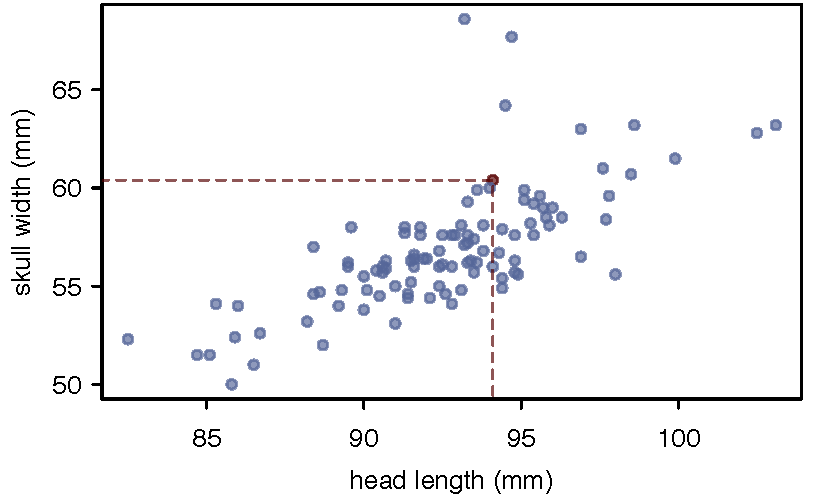
\includegraphics[width=0.7\textwidth]{01/figures/possumHeadVsSkullW/possumHeadVsSkullW}
\caption{A scatterplot showing \var{skullW} against \var{headL}. The possum with a head length of 94.1mm and a skull width of 60.4mm is highlighted.}
\label{possumHeadVsSkullW}
\end{figure}

\begin{exercise}
Examine the variables in the \data{cars} data set, which are described in Table~\ref{carsVariables} on page~\pageref{carsVariables}. Create two questions about the relationships between these variables that are of interest to you.
%Create two additional questions about the relationships between the variables that are of interest to you.
\end{exercise}

%The first question about \data{possum}, discussed above, is sort of boring. So possums with short heads tend to have slimmer skulls -- that isn't surprising! But some of the other questions might stem from a deeper question.

\subsection{Associated and independent variables}
\label{associatedAndIndependentVariablesSubsection}

The variables \var{headL} and \var{skullW} are said to be associated because the plot shows a discernible pattern. When two variables show some connection with one another, they are called \term{associated} variables. Associated variables can also be called \term{dependent} variables and vice-versa.

\begin{example}{Examine the scatterplot of \var{weight} and \var{mpgCity} in Figure~\ref{carsMpgCityVsWeight}. Are these variables associated?}
It appears that the heavier a car is, the worse mileage it gets. Since there is some relationship between the variables, they are associated.
\end{example}
\begin{figure}
   \centering
   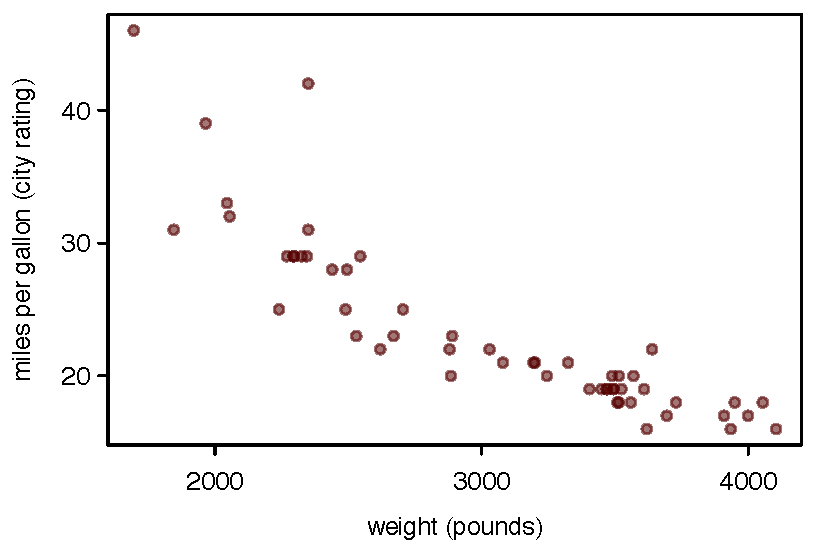
\includegraphics[width=0.7\textwidth]{01/figures/carsMpgCityVsWeight/carsMpgCityVsWeight}
   \caption{A scatterplot of \var{mpgCity} versus \var{weight} for the \data{cars} data set.}
   \label{carsMpgCityVsWeight}
\end{figure}

Because there is a downward trend in Figure~\ref{carsMpgCityVsWeight} --  larger weights are associated with lower mileage -- these variables are said to be \term{negatively associated}. A \term{positive association} is shown in the possum data represented in Figure~\ref{possumHeadVsSkullW}, where longer heads are associated with wider skulls.

If two variables are not associated, then they are said to be \term{independent}. That is, two variables are independent if there is no evident connection between the two. % In the sulphinpyrazone study, we would like to know if the patients' outcomes are independent of the treatment they received. If they are independent, this would mean the drug does not work. If they are as
It is also possible for cases -- such as a pair of possums or a pair of people -- to be independent. For instance, if possums 1 and 2 are not siblings, do not compete for resources in the same territory, and show no other natural connections, then they can be called independent.

% It is also possible for cases or individuals to be independent. For instance, if we randomly pick two possums from Australia,  will not be related 

%\begin{termBox}{\tBoxTitle{Independence}
%Two things are independent of each other if they are not associated (dependent).}
%\end{termBox}

\begin{termBox}{\tBoxTitle{Associated or independent, not both}
A pair of variables are either related in some way (associated) or not (independent). No pair of variables is both associated and independent. These same definitions hold true for a pair of cases as well.}
\end{termBox}

%Variables can be associated or independent. Cases can be associated or independent. However, a variable cannot be associated or independent of a case. For example, the \var{headL} variable cannot be independent of possum 1. In statistics, for two things to be independent of each other, they must be comparable. It makes no sense to discuss independence between a variable and a case. 

%Associations between categorical variables will be discussed in Section~\ref{categoricalData}.

\section{Examining numerical data}
\label{numericalData}

The \data{cars} data set represents a \emph{sample} from a larger set of cases. This larger set of cases is called the \term{population}. Ideally data would be collected from every case in the population. However, this is rarely possible due to high costs of data collection. As a substitute, statisticians collect subsets of the data called \termsub{samples}{sample} to gain insights into the population. The \data{cars} data set represents a sample of all cars from 1993, and the \data{possum} data set represents a sample from all possums in the Australian states of Victoria, New South Wales, and Queensland. In this section we introduce summary statistics and graphics as a first step in analyzing numerical data from a sample to help us understand certain features of the population as a whole.

\subsection{Scatterplots for paired data}
\label{scatterPlots}

A \term{scatterplot} provides a case-by-case view of data for two numerical variables. In Section~\ref{variableRelations}, a scatterplot was used to examine how head length and skull width were related in the \data{possum} data set. Another scatterplot is shown in Figure~\ref{carsPriceVsWeight}, comparing \var{price} and \var{weight} for the \data{cars} data set.
\begin{figure}[h]
   \centering
   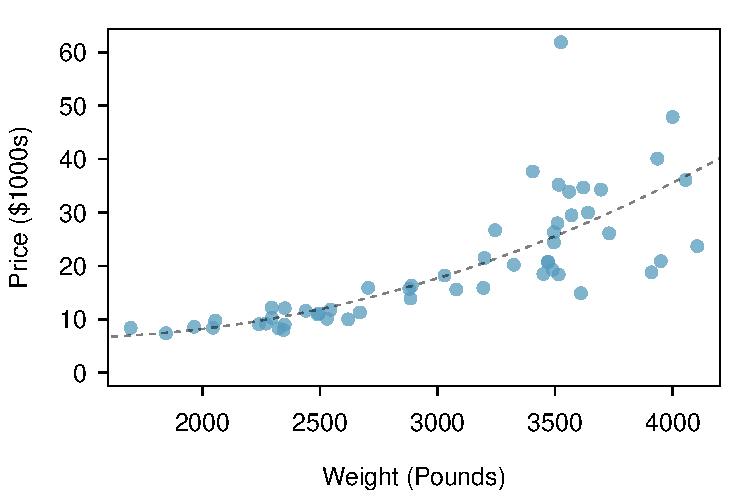
\includegraphics[height=2.6in]{01/figures/carsPriceVsWeight/carsPriceVsWeight}
   \caption{A scatterplot of \var{price} versus \var{weight} for the \data{cars} data set.}
   \label{carsPriceVsWeight}
\end{figure}

In any scatterplot, each point represents a single case. Since there are 54 cases in \data{cars}, there are 54 points in Figure~\ref{carsPriceVsWeight}.

\begin{exercise}
What do scatterplots reveal about the data, and how might they be useful?
\end{exercise}

Some associations are more linear, like the relationship between \var{skullW} and \var{headL}, shown in Figure~\ref{possumHeadVsSkullW} on page~\pageref{possumHeadVsSkullW}. Others, like the one seen in Figure~\ref{carsMpgCityVsWeight} can be curved.

\begin{exercise}
Describe two variables that would have a horseshoe shaped association in a scatterplot. One example is given in the footnote\footnote{Consider the case where your vertical axis represents something ``good'' and your horizontal axis represents something that is only good in moderation. Health and water consumption fit this description since water becomes toxic when consumed in excessive quantities.}.
\end{exercise}

\subsection{Dot plots and the mean}
\label{dotPlot}

Sometimes two variables is one too many: only one variable may be of interest. In these cases, a dot plot provides the most basic of displays. A dot plot is a one-variable scatterplot, and a sample dot plot is shown in Figure~\ref{carsPriceDotPlot}.
\begin{figure}[h]
   \centering
   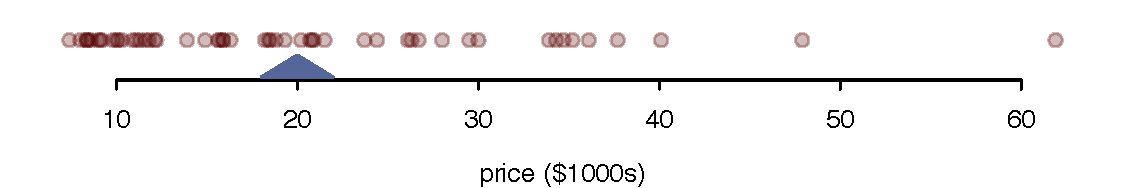
\includegraphics[width=\textwidth]{01/figures/carsPriceDotPlot/carsPriceDotPlot}
   \caption{A dot plot of \var{price} for the \data{cars} data set. The triangle marks the sample's mean price.}
   \label{carsPriceDotPlot}
\end{figure}

The \term{mean}, sometimes called the average, is a way to measure the center of a \term{distribution} of data. To find the mean price of the cars in the sample, add up all the prices and divide by the number of cases.
\begin{eqnarray}
\bar{x} = \frac{15.9 + 33.9 + \cdots + 26.7}{54} = 19.99259
\label{sampleMeanEquation}
\end{eqnarray}
The sample mean is often labeled $\bar{x}$\marginpar[\raggedright$\bar{x}$\\\footnotesize sample\\ mean]{\raggedright$\bar{x}$\\\footnotesize sample\\ mean}. The letter $x$ is being used as an abbreviation for \var{price}, and the bar says it is the sample average of price. It is useful to think of the mean as the balancing point of the distribution. The sample mean is shown as a blue triangle in Figure~\ref{carsPriceDotPlot}.

\begin{termBox}{\tBoxTitle{Mean}
The sample mean of a numerical variable is computed as the sum of all of the observations divided by the number of observations:
\begin{eqnarray}
\bar{x} = \frac{x_1+x_2+\cdots+x_n}{n}
\label{meanEquation}
\end{eqnarray}
where $x_1, x_2, \dots, x_n$ represent the $n$ observed values.}
\end{termBox}\marginpar[\raggedright\vspace{-8mm}

$n$\\\footnotesize sample size]{\raggedright\vspace{-8mm}

$n$\\\footnotesize sample size}\vspace{-2mm}

\begin{exercise}
Examine equations~(\ref{sampleMeanEquation}) and~(\ref{meanEquation}) above. What does $x_1$ correspond to? And $x_2$? Can you infer a general meaning to what $x_i$ might represent? Answers in the footnote\footnote{$x_1$ corresponds to the price of the first car (15.9), $x_2$ to the price of the second car (33.9), and $x_i$ corresponds to the price of the $i^{th}$ car in the data set.}.
\end{exercise}

\begin{exercise}
What was $n$ in the \data{cars} data set? Answer in the footnote\footnote{The sample size is $n=54$.}.
\end{exercise}

The \emph{population} mean is also computed in the same way, however, it has a special label: $\mu$. The symbol $\mu$\marginpar[\raggedright$\mu$\\\footnotesize population\\ mean]{\raggedright$\mu$\\\footnotesize population\\ mean} is the Greek letter \emph{mu} and represents the average of all observations in the population. Sometimes a subscript, such as $_x$, is used to represent which variable the population mean refers to, i.e. $\mu_x$.

\begin{example}{The average price of all cars from 1993 can be estimated using the sample data. Based on the \data{cars} sample, what would be a reasonable estimate of $\mu_x$, the mean price of cars from 1993?}
The sample mean may provide a good estimate of $\mu_x$. While this estimate will not be perfect, it provides a \emph{point estimate} of the population mean.
\end{example}

\subsection{Histograms and shape}
\label{histogramsAndShape}

Dot plots show the exact value for each observation. This is useful for small data sets, but can become problematic for larger samples. Rather than showing the value of each observation, we might prefer to think of the value as belonging to a \emph{bin}. For example, in the \data{cars} data set, we could create a table of counts for the number of cases with prices between \$5,000 and \$10,000, then the number of cases between \$10,000 to \$15,000, and so on. Observations that fall on the boundary of a bin (e.g. \$10,000) are allocated to the lower bin. This tabulation is shown in Table~\ref{binnedCarsPriceTable}. To make the data easier to see visually, these binned counts are plotted as bars in Figure~\ref{carsPriceHist}. This binned version of the dot plot is called a \term{histogram}.
\begin{table}[ht]
\centering\small
\begin{tabular}{l ccc ccc ccc}
  \hline
Price & 5-10 & 10-15 & 15-20 & 20-25 & 25-30 & 30-35 & $\cdots$ & 55-60 & 60-65 \\
  \grayline
Count & 11 &  11 &  10 &   7 &   6 &   3 & $\cdots$ & 0 & 1 \\
  \hline
\end{tabular}
\caption{The counts for the binned \var{price} data, where \var{price} is in thousands of dollars.}
\label{binnedCarsPriceTable}
\end{table}
\vspace{-2mm}
\begin{figure}[bth]
   \centering
   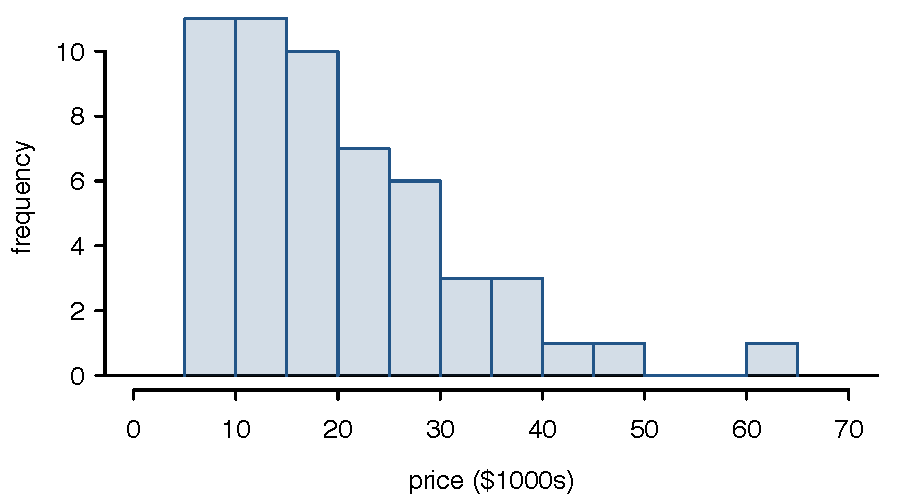
\includegraphics[width=0.75\textwidth]{01/figures/carsPriceHist/carsPriceHist}
   \caption{Histogram of \var{price}.}
   \label{carsPriceHist}
\end{figure}

Histograms provide a view of the \term{data density}. Higher bars represent where the data are relatively more common. For instance, there are many more cars that cost less than \$15,000 than cars that cost at least \$50,000 in the data set. The bars make it especially easy to see how the density of the data changes from one price to another: in general, the higher the price, the fewer the cars.

Histograms are especially convenient for describing the shape of the data distribution\label{shapeFirstDiscussed}. Figure~\ref{carsPriceHist} shows that most cars have a lower price, while fewer cars have higher prices. When data trail off to the right in this way and have a longer right \hiddenterm{tail}, the shape is said to be \term{skewed to the right}\footnote{Other ways to describe data skewed to the right: \term{right skewed}, \term{skewed to the high end}, or \term{skewed to the positive end}.}.

Data sets with the reverse characteristic -- a long, thin tail to the left -- are said to be \term{left skewed}. It might also be said that such a distribution has a long left tail. Data sets that show roughly equal trailing off in both directions are called \term{symmetric}.

\begin{termBox}{\tBoxTitle{Long tails to identify skew}
When data trail off in one direction, it is called a \term{long tail}. If a distribution has a long left tail, it is left skewed. If a distribution has a long right tail, it is right skewed.}
\end{termBox}

\begin{exercise}
Take a look at Figure~\ref{carsPriceDotPlot} on page~\pageref{carsPriceDotPlot}. Can you see the skew in the data? Is it easier to see the skew in Figure~\ref{carsPriceDotPlot} or Figure~\ref{carsPriceHist}?
\end{exercise}

\begin{exercise}
Besides the mean (since it was labeled), what can you see in Figure~\ref{carsPriceDotPlot} that you cannot see in \ref{carsPriceHist}? Answer in the footnote\footnote{The individual prices.}.
\end{exercise}

In addition to looking at whether a distribution is skewed or symmetric, histograms can be used to identify modes. A \term{mode} is represented by a prominent peak in the distribution\footnote{Another definition of mode, which is not typically used in statistics, is the value with the most occurrences. It is common to have \emph{no} observations with the same values in a data set, which makes this other definition useless for many real data sets.}. There is only one prominent peak in the histogram of \var{price}.

Figure~\ref{singleBiMultiModalPlots} shows histograms that have one, two, and three prominent peaks. Such distributions are called \term{unimodal}, \term{bimodal}, and \term{multimodal}, respectively. Any distribution with more than 2 prominent peaks is called multimodal. Notice that there was one prominent peak in the unimodal distribution with a second less prominent peak that was not counted since it only differs from its neighboring bins by a few observations.
\begin{figure}[h]
   \centering
   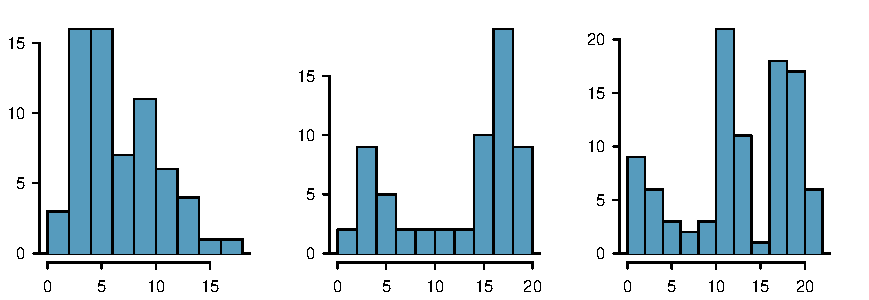
\includegraphics[width=\textwidth]{01/figures/singleBiMultiModalPlots/singleBiMultiModalPlots}
   \caption{Counting only prominent peaks, the distributions are (left to right) unimodal, bimodal, and multimodal.}
   \label{singleBiMultiModalPlots}
\end{figure}

\begin{exercise}
Figure~\ref{carsPriceHist} reveals only one prominent mode in \var{price}. Is the distribution unimodal, bimodal, or multimodal?
\end{exercise}

\begin{exercise}
Height measurements of young students and adult teachers at a K-3 elementary school were taken. How many modes would you anticipate in this height data set? Answer in the footnote\footnote{There might be two height groups visible in the data set: one of the students and one of the adults. That is, the data might be bimodal.}.
\end{exercise}

\begin{tipBox}{\tipBoxTitle{Looking for modes}
Looking for modes isn't about finding a clear and correct answer about the number of modes in a distribution, which is why \emph{prominent} is not defined mathematically here. The importance of this examination is to better understand your data and how it might be structured.}
\end{tipBox}

%If you find two or more prominent peaks, the data may arise from two or more subpopulations. Even if the distribution is not bimodal or multimodal, it is certainly not uncommon to reap benefits from grouping data by other variables, which will be discussed casually in Section~\ref{comparingAcrossGroups}.

\subsection{Variance and standard deviation}
\label{variability}

The mean was introduced as a method to describe the center of a data set but the data's variability is also important. Here, we introduce two measures of variability: the variance and the standard deviation. Both of these are very useful in data analysis, even though their formulas are a bit tedious to compute by hand.

We call the distance of an observation from its mean its \term{deviation}. Below are the $1^{st}_{}$, $2^{nd}_{}$, and $54^{th}_{}$ deviations for the \var{price} variable:
\begin{align*}
x_1^{}-\bar{x} &= 15.9-20 = -4.1 \hspace{5mm}\text{ } \\
x_2^{}-\bar{x} &= 33.9-20 = 13.9 \\
			&\ \vdots \\
x_{54}^{}-\bar{x} &= 26.7-20 = 6.7
\end{align*}
If we square these deviations and then take an average, the result is about equal to the sample \term{variance}\label{varianceIsDefined}, denoted by $s_{}^2$\marginpar[\raggedright$s^2_{}$\\\footnotesize sample variance]{\raggedright$s^2_{}$\\\footnotesize sample variance}:
\begin{eqnarray*}
s_{}^2 = \frac{(-4.1)_{}^2 + (13.9)_{}^2 + \cdots + (6.7)_{}^2}{54-1} = \frac{16.8 + 193.2 + \cdots + 44.9}{53} = 132.4
\end{eqnarray*}
(We divide by $n-1$ (rather than dividing by $n$) when computing the variance.) % for reasons described in the footnote\footnote{The population of all cars from 1993 has some precise variance in vehicle prices. Our estimate of this variance tends to be slightly better if we divide by $n-1$ instead of $n$.}
Notice that squaring the deviations does two things: (i) it makes large values much larger, seen by comparing $(-4.1)^2$, $13.9^2$, and $6.7^2$, and (ii) it gets rid of any negative signs.
%We divide by $n-1$ instead of $n$ for reasons described in the footnote\footnote{The population of all cars from 1993 has some precise variance in vehicle prices. Our estimate of this variance tends to be slightly better if we divide by $n-1$ instead of $n$.}. Notice that squaring the deviations does two things: (i) it makes large values much larger, seen by comparing $(-4.1)^2$, $13.9^2$, and $6.7^2$, and (ii) it gets rid of any negative signs.

The \term{standard deviation} is defined as the square root of the variance:
$$s=\sqrt{132.4} = 11.5$$
\marginpar[\raggedright\vspace{-10mm}

$s$\\\footnotesize sample standard deviation]{\raggedright\vspace{-10mm}

$s$\\\footnotesize sample standard deviation}
A subscript of $_x$ may be added to the the variance and standard deviation -- that is, $s_x^2$ and $s_x^{}$ -- as a reminder that these are the variance and standard deviation of the observations represented by $x_1^{}$, $x_2^{}$, ..., $x_n^{}$. These may be omitted when it is clear which data the standard deviation is referencing.

\begin{termBox}{\tBoxTitle{Variance and standard deviation}
The variance is roughly the average squared distance from the mean. The standard deviation is the square root of the variance.}
\end{termBox}

Formulas and methods used to compute the variance and standard deviation for a population are similar to those used for a sample\footnote{The only difference is that the population variance has a division by $n$ instead of $n-1$.}. However, like the mean, the population values have special symbols: $\sigma_{}^2$\marginpar[\raggedright$\sigma_{}^2$\\\footnotesize population variance\\ \hspace{2mm}]{\raggedright$\sigma_{}^2$\\\footnotesize population variance\\ \hspace{2mm}} for the variance and $\sigma$\marginpar[\raggedright$\sigma$\\\footnotesize population standard deviation\\ \hspace{2mm}]{\raggedright$\sigma$\\\footnotesize population standard deviation\\ \hspace{2mm}} for the standard deviation. The symbol $\sigma$ is the Greek letter \emph{sigma}. As with the sample variance and standard deviation, subscripts such as $_{x}^{}$ can be added to specify which data sets the population variance and standard deviation reference.
\begin{figure}
\centering
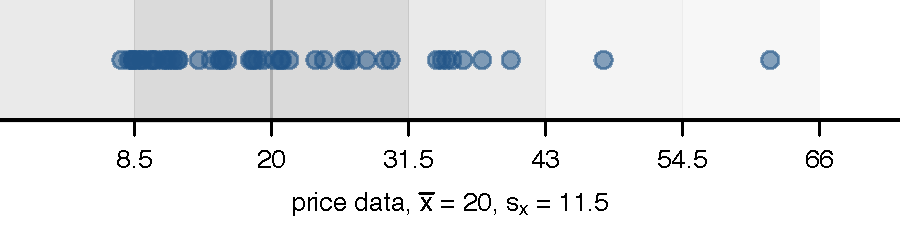
\includegraphics[width=\mycaptionwidth]{01/figures/sdAsRuleForCarsPrice/sdAsRuleForCarsPrice}
\caption{In the \var{price} data, 40 of 54 cars (74\%) are within 1 standard deviation of the mean, \$20,000. Additionally, 52 of the 54 cars (96\%) and 53 of the 54 prices (98\%) are within 2 and 3 standard deviations, respectively.}
\label{sdAsRuleForCarsPrice}
\end{figure}

The standard deviation is useful in considering how close the data are to the mean. Usually about 70\% of the data are within one standard deviation of the mean and 95\% within two standard deviations. However, these percentages can and do vary from one distribution to another. Figure~\ref{severalDiffDistWithSdOf1} shows several different distributions that have the same center and variability but very different shapes.
\begin{figure}
\centering
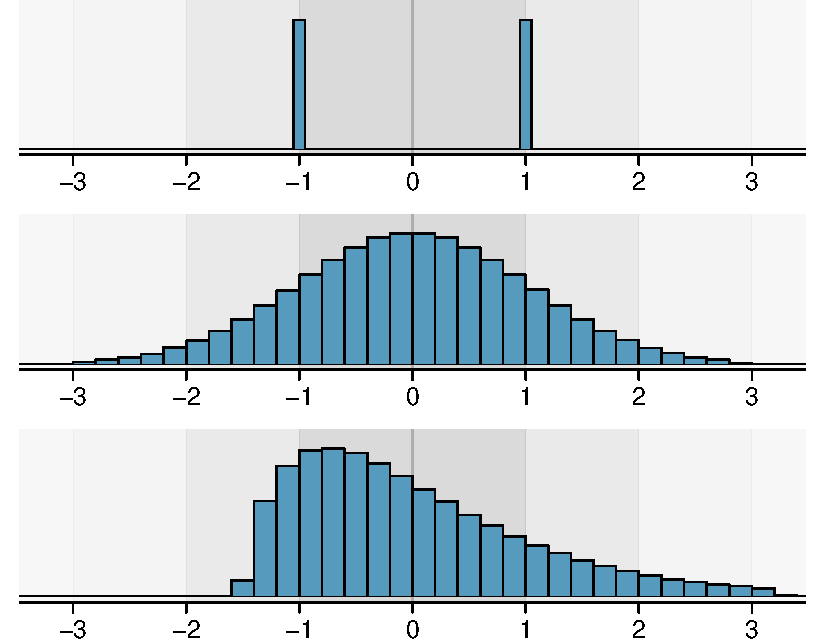
\includegraphics[width=0.65\textwidth]{01/figures/severalDiffDistWithSdOf1/severalDiffDistWithSdOf1}
\caption{Three very different population distributions with the same mean $\mu=0$ and standard deviation $\sigma=1$.\vspace{-3mm}}
\label{severalDiffDistWithSdOf1}
\end{figure}

\begin{exercise}
On page~\pageref{shapeFirstDiscussed}, the concept of shape of a distribution was introduced. A good description of the shape of a distribution should include modality and whether the distribution is symmetric or skewed to one side. Using Figure~\ref{severalDiffDistWithSdOf1} as an example, explain why such a description is important.
\end{exercise}

\begin{example}{Describe the distribution of the \var{price} variable, shown in Figure~\ref{carsPriceHist} on page~\pageref{carsPriceHist}. The description should incorporate the center, variability, and shape of the distribution, and it should also be placed in context of the problem: the price of cars. Also note any especially unusual cases.}
The distribution of car prices is unimodal and skewed to the high end. Many of the prices fall near the mean at \$20,000, and most fall within one standard deviation (\$11,500) of the mean. There is one very expensive car that costs more than \$60,000.
\end{example}

%; a very peculiar distribution might have no data within one standard deviation or only 75\% of the data within two standard deviations. %, For instance, it is guaranteed that no more than $\frac{1}{2^2}=1/4^{th}$ of the data will be further than 2 standard deviations from the mean. Likewise, at most $\frac{1}{3^2}=1/9^{th}$ of the data can be further than 3 standard deviations. The Theorem in the footnote provides the general rule\footnote{Chebyshev's Theorem: No more than a fraction $1/k^2$ of the data can be further than $k$ standard deviations from the mean. This rule is conservative for many data sets.}.

%These approximate guidelines do not give the only use of the standard deviation (and variance), however, the other applications are too obscure to go into detail here. 
In practice, the variance and standard deviation are sometimes used as a means to an end, where the ``end'' is being able to accurately estimate the uncertainty associated with a sample statistic. For example, in Chapter~4 %ZZQ \ref{foundationsForInference}
we use the variance and standard deviation to assess how close the sample mean is to the population mean.

\begin{tipBox}{\tipBoxTitle{standard deviation describes variability}
Standard deviation is complex mathematically. However, it is not conceptually difficult. %: it provides a useful measure of the variability in a data set.
It is useful to remember that usually about 70\% of the data are within one standard deviation of the mean and about 95\% are within two standard deviations.}
\end{tipBox}


%This rule does not provide the only use of the standard deviation, which provides a solid foundation for understanding variability in the data. In practice, the variance and standard deviation are many times a means to an end, and the ``end'' is being able to accurately estimate the uncertainty associated with an estimate. For example, the variance and standard deviation are useful in determining how close one should anticipate the sample mean is to the population mean. We will continue to be discuss variance and standard deviation over the next few chapters while the details of its common use will be introduced in Chapter~\ref{foundationsForInference} and beyond.

\subsection{Box plots, quartiles, and the median}

A box plot summarizes a data set using five statistics while also plotting unusual observations. Figure~\ref{boxPlotLayout} provides a vertical dot plot alongside a box plot of the \var{price} variable from the \data{cars} data set.
\begin{figure}[h]
   \centering
   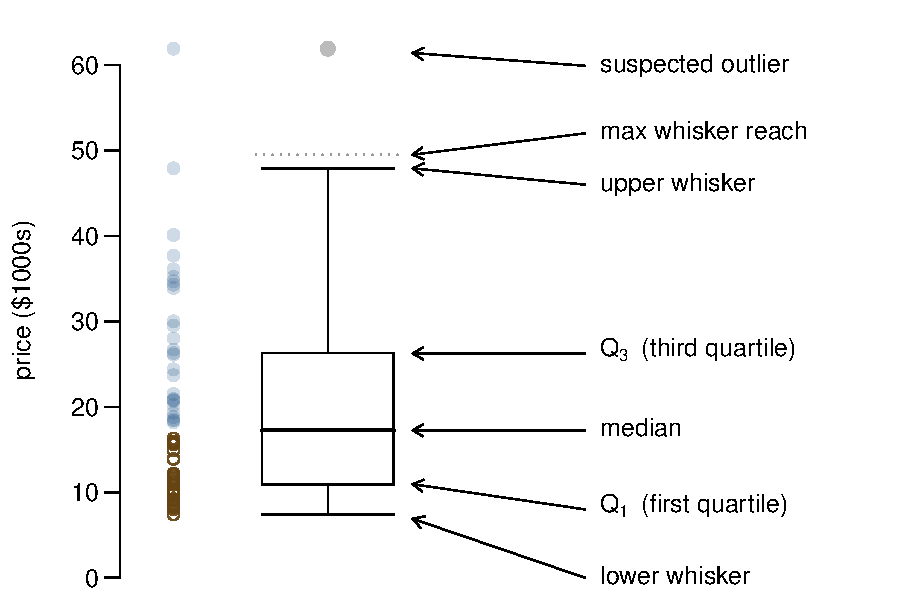
\includegraphics[height=2.8in]{01/figures/boxPlotLayout/boxPlotLayout}
   \caption{A vertical dot plot next to a labeled box plot of the \var{price} data. The median (\$17,250), splits the data into the bottom 50\% and the top 50\%, marked in the dot plot by dark-colored hollow circles and light filled circles, respectively.}
   \label{boxPlotLayout}
\end{figure}

The first step in building a box plot is drawing a rectangle to represent the middle 50\% of the data. The total length of the box, shown vertically in Figure~\ref{boxPlotLayout}, is called the \term{interquartile range} (IQR, for short). It, like the standard deviation, is a measure of variability in data. The more variable the data, the larger the standard deviation and IQR. The two boundaries of the box are called the \term{first quartile} (the $25^{th}$ \hiddenterm{percentile}, i.e. 25\% of the data fall below this value) and the \term{third quartile} (the $75^{th}$ percentile), and these are often labeled $Q_1$ and $Q_3$, respectively.

\begin{termBox}{\tBoxTitle{Interquartile range (IQR)}
The \term{interquartile range (IQR)} is the length of the box in a box plot. It is computed as
\begin{eqnarray*}
IQR = Q_3 - Q_1
\end{eqnarray*}
where $Q_1$ and $Q_3$ are the $25^{th}$ and $75^{th}$ percentiles.}
\end{termBox}

The line splitting the box denotes the \term{median}, or the value that splits the data in half. Figure~\ref{boxPlotLayout} shows 50\% of the data falling below the median (dark hollow circles) and other 50\% falling above the median (light-colored filled circles). There are 54 car prices in the data set (an even number) so the data are perfectly split into two groups of 27. We take the median in this case to be the average of the two observations closest to the $50^{th}$ percentile: $\frac{\$16,300 + \$18,200}{2} = \$17,250$. When there are an odd number of observations, there will be exactly one observation that splits the data into two halves, and in this case that observation is the median (no average needed).

%The line splitting the box marks the \term{median}, or the ``middle'' observation in the data. Half of the observations fall below the median and half are above. In the \data{cars} data set, there are 54 car prices, in which case  in the data set and the $27^{th}$ and $28^{th}$ largest observations (the middle observations) are \$16,300 and \$18,200. Because this represents a tie for the middle number, the median is taken as the average of the two: \$17,250. \\


\begin{termBox}{\tBoxTitle{Median: the number in the middle}
If the data are ordered from smallest to largest, the \term{median} is the observation right in the middle. If there are an even number of observations, there will be two values in the middle, and the median is taken as their average.}
\end{termBox}

\begin{exercise}
What percent of the data fall between $Q_1$ and the median? How much between the median and $Q_3$? Answers in the footnote\footnote{Since $Q_1$ and $Q_3$ capture the middle 50\% of the data and the median splits the data in the middle, 25\% of the data fall between $Q_1$ and the median, and another 25\% falls between the median and $Q_3$.}.
\end{exercise}

Extending out from the box, the \term{whiskers} attempt to capture the data outside of the box, however, their reach is never allowed to be more than $1.5*IQR$.\footnote{While the choice of exactly 1.5 is arbitrary, it is the most commonly used value for box plots.} They grab everything within this reach. In Figure~\ref{boxPlotLayout}, the upper whisker cannot extend to the last point, which is beyond $Q_3 + 1.5*IQR$, and so it extends only to the last point below this limit. The lower whisker stops at the lowest price, \$7,400, since there is no additional data to reach; the lower whisker limit is not shown in the figure because the plot does not extend down to $Q_1 - 1.5*IQR$. In a sense, the box is like the body of the box plot and the whiskers are like its arms trying to reach the rest of the data.

Any observation that lies beyond the whiskers is labeled with a dot. The purpose of labeling these points -- instead of just extending the whiskers to the minimum and maximum observed values -- is to help identify any observations that appear to be unusually distant from the rest of the data. Unusually distant observations are called \term{outliers}. In the case of the \var{price} variable, the car with price \$61,900 is a potential outlier.

\begin{termBox}{\tBoxTitle{Outliers are extreme}
An \term{outlier} is an observation that appears extreme relative to the rest of the data.}
\end{termBox}


\begin{tipBox}{\tipBoxTitle{Why it is important to look for outliers}
Examination of data for possible outliers serves many useful purposes, including\vspace{-2mm}
\begin{enumerate}
\setlength{\itemsep}{0mm}
\item Identifying extreme skew in the distribution.
%\item Inferring that seemingly unusual cases are actually commonplace for a variable.
\item Identifying data collection or entry errors. If there was a car price listed as \$140,000, it would be worth reviewing the observation to see whether it was really \$14,000.
\item Providing insights into interesting phenomena with the data.
\end{enumerate}}
%The identification of outliers is not actually what is important, which is why no rigid definition for outlier is provided. What is important is to examine and take special note of \emph{suspected} outliers and why they are extreme compared to the rest of the data.}
\end{tipBox}

\begin{exercise}
The observation \$61,900, a suspected outlier, was found to be an accurate observation. What would such an observation suggest about the nature of vehicle prices?
\end{exercise}

\begin{exercise}
Using Figure~\vref{boxPlotLayout}, estimate the following values for \var{price} in the \data{cars} data set: (a) $Q_1$, (b) $Q_3$, and (c) IQR.
\end{exercise}

\subsection{Robust statistics}

How would sample statistics of the \data{cars} data set be affected if \$200,000 was observed instead of \$61,900 for the most expensive car? Or what if \$200,000 had been in the sample instead of the cheapest car at \$7,400? These two scenarios are plotted alongside the original data in Figure~\ref{carsPriceDotPlotRobustEx}, and sample statistics are computed under each of these scenarios in Table~\ref{robustOrNotTable}.
\begin{figure}[ht]
\centering
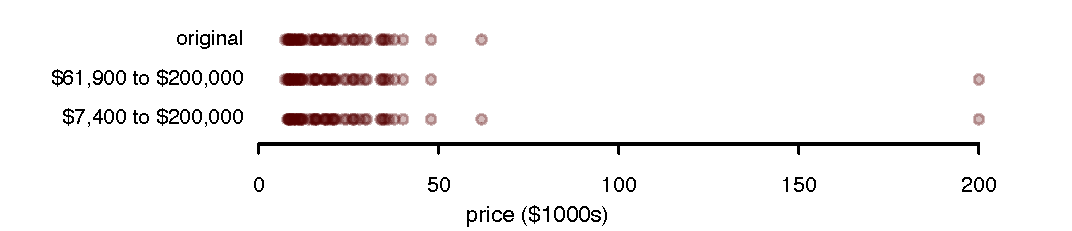
\includegraphics[width=\textwidth]{01/figures/carsPriceDotPlotRobustEx/carsPriceDotPlotRobustEx}
\caption{Dot plots of the original price data and two modified price data sets.}
\label{carsPriceDotPlotRobustEx}
\end{figure}
\begin{table}[ht]
\centering
\begin{tabular}{l c cc c cc}
  \hline
& \hspace{0mm} & \multicolumn{2}{c}{\bf robust} & \hspace{2mm} & \multicolumn{2}{c}{\bf not robust} \\
scenario && median & IQR && $\bar{x}$ & $s$ \\ 
  \hline
original \var{price} data && 17.25 & 15.30 && 19.99 & 11.51 \\ 
move \$61,900 to \$200,000 && 17.25 & 15.30 && 22.55 & 26.53 \\ 
move \$7,400 to \$200,000 && 18.30 & 15.45 && 26.12 & 35.79 \\ 
   \hline
\end{tabular}
\caption{A comparison of how the median, IQR, mean ($\bar{x}$), and standard deviation ($s$) change when extreme observations are in play.}
\label{robustOrNotTable}
\end{table}

\begin{exercise}
(a) Which is more affected by extreme observations, the mean or median? Table~\ref{robustOrNotTable} may be helpful. (b) Is the standard deviation or IQR more affected by extreme observations?
\end{exercise}

The median and IQR are called \term{robust estimates} because extreme observations have little effect on their values. The mean and standard deviation are much more affected by changes in extreme observations.

\begin{exercise}
Why doesn't the median or IQR change from the original \var{price} data to the second scenario of Table~\ref{robustOrNotTable}?
\end{exercise}

%\begin{exercise}
%Are the extreme changes in the mean and standard deviation a fluke? Look back to how the mean and standard deviation are actually computed on pages~\pageref{meanEquation} and~\pageref{varianceIsDefined}. Why is it that these two variables are affected by (suspected) outliers, i.e. observations that are far from the rest of the data? Compare this with how the median and IQR are computed.
%\end{exercise}

\begin{exercise}
Why are robust statistics useful? If you were searching for a new car and cared about price, would you be more interested in the mean vehicle price or the median vehicle price when considering the price for a regular car?
\end{exercise}

\subsection{Transforming data (special topic)}

When data are extremely skewed, we sometimes transform them so they are easier to model. Consider the histogram of salaries for Major League Baseball players' salaries from 2010, which is shown in Figure~\ref{histMLBSalariesReg}. %, and Figure~\ref{histMLBSalariesReg} shows the same data set after a log transformation.
\begin{figure}[ht]
\centering
\subfigure[]{
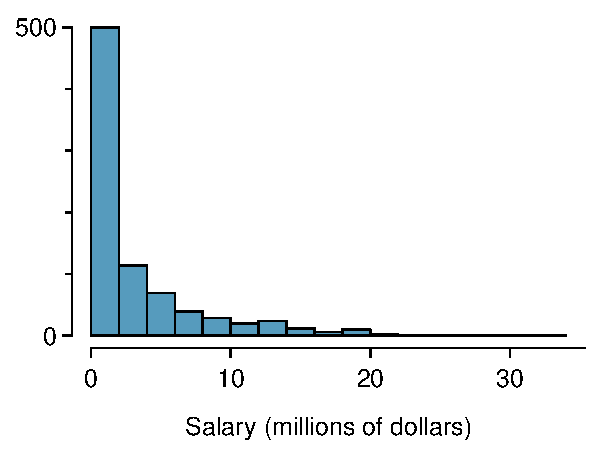
\includegraphics[width=0.46\textwidth]{01/figures/histMLBSalaries/histMLBSalariesReg}
\label{histMLBSalariesReg}
}
\subfigure[]{
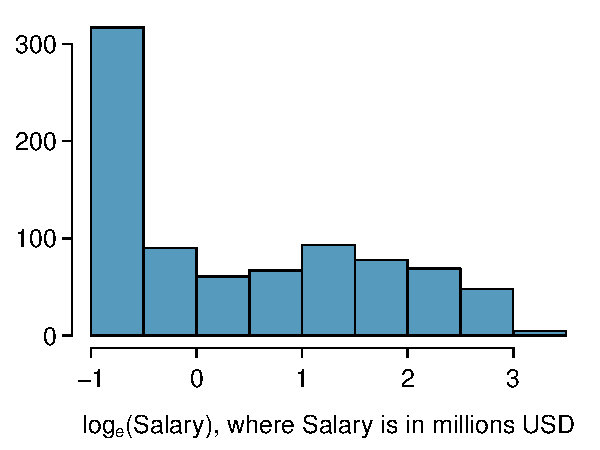
\includegraphics[width=0.46\textwidth]{01/figures/histMLBSalaries/histMLBSalariesLog}
\label{histMLBSalariesLog}
}
\caption{\subref{histMLBSalariesReg} Histogram of MLB player salaries for 2010, in millions of dollars. \subref{histMLBSalariesLog} Histogram of the log-transformed MLB player salaries for 2010.}
\label{histMLBSalaries}
\end{figure}

\begin{example}{The histogram of MLB player salaries is useful in that we can see the data are highly skewed and centered (as gauged by the median) at about \$1 million. What isn't useful about this plot?}
Most of the data are collected into one bin in the histogram and the data are so strongly skewed that some details in the data are obscured.
\end{example}

There are some standard transformations that are often applied when much of the data cluster near zero (relative to the larger values in the data set) and all observations are positive. A \term{transformation} is a rescaling of the data using a function. For instance, a plot of the natural logarithm\footnote{Statisticians often write the natural logarithm as $\log$. You might be more familiar with it being written as $\ln$.} of player salaries results in a new histogram in Figure~\ref{histMLBSalariesLog}. Transformed data are sometimes easier to work with when applying statistical models because the transformed data are much less skewed and outliers are usually less extreme. %The extreme skew in the pre-transformed data was so strong that it would add an extra layer of modeling complexity.

%\begin{exercise}
%What do you notice in Figure~\ref{histMLBSalariesReg} that you were unable to see in Figure~\ref{histMLBSalariesLog}?
%\end{exercise}

Transformations can also be applied to one or both variables in a scatterplot. A scatterplot is shown in Figure~\ref{scatterMammalGestLSReg} representing mammal lifespans against the time of gestation (time spent in the womb). There seems to be a positive association between these two variables. In Chapter~7, %ZZQ\ref{},
we might want to use a straight line to model the data. However, we'll find that the data in their current state cannot be modeled very well. Figure~\ref{scatterMammalGestLSTra} shows a scatterplot where both the \var{gestation} and \var{lifespan} variables have been transformed using a log (base $e$) transformation. While there is a positive association in each plot, the transformed data show a steadier trend, which is easier to model than the untransformed data.
\begin{figure}
\centering
\subfigure[]{
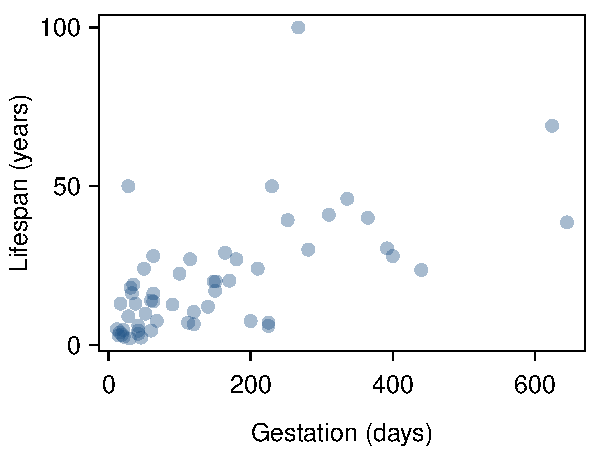
\includegraphics[width=0.46\textwidth]{01/figures/scatterMammalGestLS/scatterMammalGestLSReg}
\label{scatterMammalGestLSReg}
}
\subfigure[]{
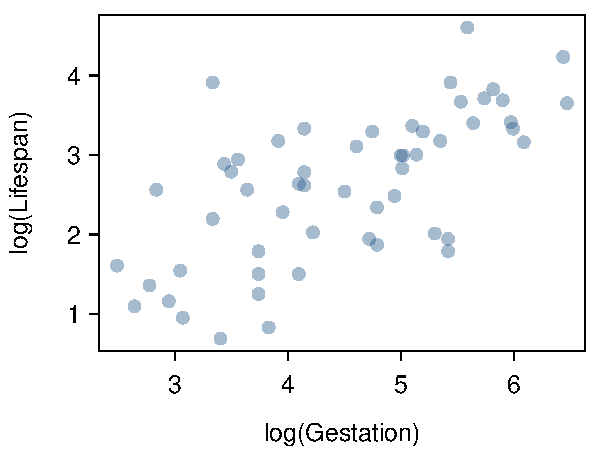
\includegraphics[width=0.46\textwidth]{01/figures/scatterMammalGestLS/scatterMammalGestLSTra}
\label{scatterMammalGestLSTra}
}
\caption{\subref{scatterMammalGestLSReg} Scatterplot of \var{Lifespan} against \var{Gestation} for 55 mammals. \subref{scatterMammalGestLSTra} A scatterplot of the same data but where each variable has been log-transformed.}
\label{scatterMammalGestLS}
\end{figure}

Other transformations other than the logarithm can be useful, too. For instance, the square root ($\sqrt{\text{original observation}}$) and inverse ($\frac{1}{\text{original observation}}$) are regularly used by statisticians. Common goals in transforming data are to see the data structure differently, reduce skew, assist in modeling, or straighten a nonlinear relationship in a scatterplot.

\section{Considering categorical data}
\label{categoricalData}

Like numerical data, categorical data can also be organized and analyzed. %In Section~\ref{basicExampleOfSulphinpyrazone}, we summarized the results of 1475 patients with variables \var{group} and \var{outcome}, both categorical variables, in a small table.
In this section, tables and other basic tools for categorical data analysis are introduced that will be used throughout this book.

\subsection{Contingency tables}

Table~\ref{typeDriveTrainTableTotals} summarizes two variables from the \data{cars} data set: \var{type} and \var{drivetrain}. A table that summarizes data for two categorical variables in this way is called a \term{contingency table}. Each number in the table represents the number of times a particular combination of variable outcomes occurred. For example, the number 19 corresponds to the number of cars in the data set that are small \emph{and} have front wheel drive. Row and column totals are also included. The \term{row totals} equal the total counts across each row (e.g. $19+0+2=21$), and \term{column totals} are total counts down each column.

A table for a single variable is called a \term{frequency table}. Table~\ref{typeContTable} is a frequency table for the \var{type} variable. If we replaced the counts with percentages or proportions, the table would be called a \term{relative frequency table}.

\begin{table}[ht]
\centering
\begin{tabular}{l | ccc | r}
  \hline
 & front & rear & 4WD & total \\ 
  \hline
small &  19 &   0 & 2 & 21 \\ 
midsize &  17 &  5 & 0 & 22 \\ 
large &   7 &   4 & 0 & 11 \\ 
   \hline
total & 43 & 9 & 2 & 54 \\
   \hline
\end{tabular}
\caption{A contingency table for \var{type} and \var{drivetrain}.}
\label{typeDriveTrainTableTotals}
\end{table}

\begin{table}[htb]
\centering
\begin{tabular}{ccc}
  \hline
small & midsize & large \\ 
  \grayline
21 &  22 &  11 \\ 
   \hline
\end{tabular}
\caption{A frequency table for the \var{type} variable.}
\label{typeContTable}
\end{table} % xtable(matrix(table(cars[,c('type')])[c(4,3,2)], nrow=1))

\begin{exercise}
Why is Table~\ref{typeContTable} redundant if Table~\ref{typeDriveTrainTableTotals} is provided?
\end{exercise}

\subsection{Bar plots and proportions}

A bar plot is a common way to display a single categorical variable. The left panel of Figure~\ref{typeBarPlot} shows a \term{bar plot} for the vehicle type. In the right panel, the counts were converted into proportions (e.g. $21/54=0.389$ for \var{small}), 
%making it easy to compare how about often different outcomes occur irrespective of sample size.
showing the fraction of the whole that are in each category.
\begin{figure}[bht]
   \centering
   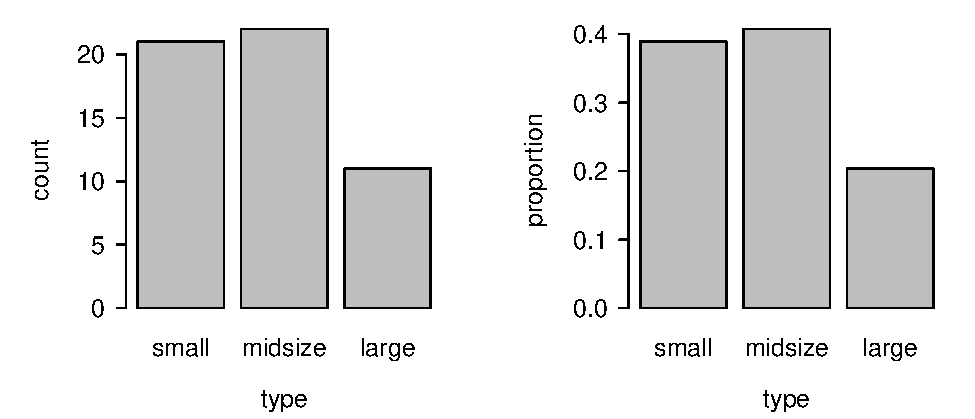
\includegraphics[height=2.3in]{01/figures/typeBarPlot/typeBarPlot}
   \caption{Two bar plots of \var{type}. The left panel shows the counts and the right panel the proportions in each group.}
   \label{typeBarPlot}
\end{figure}

\begin{exercise}
Which of the following statements would be more useful to an auto executive? (1) 21 cars in our sample were small vehicles. (2) 38.9\% of the cars in our sample were small vehicles. Comment in the footnote\footnote{Even if the sample size (54) was provided in the first statement, the auto exec would probably just be trying to figure out the proportion in her head.}.
\end{exercise}

%\begin{tipBox}{\tipBoxTitle{data set notation}
%Sometimes the values \resp{1} and \resp{0} are used as the outcomes for a categorical variable if it only has two levels. For instance, if there were only \resp{small} and \resp{large} cars, we could have used \resp{1} to represent \resp{small} and \resp{0} to represent \resp{large} in the \var{type} variable.}
%\end{tipBox}

Table~\ref{rowPropTypeDriveTrain} shows the row proportions for Table~\ref{typeDriveTrainTableTotals}. The \term{row proportions} are computed as the counts divided by their row totals. The count 17 at the intersection of \resp{midsize} and \resp{front} is replaced by $17/22=0.773$, i.e. 17 divided by its row total, 22. So what does 0.773 represent? It corresponds to the proportion of midsize vehicles in the sample that have front wheel drive.
\begin{table}[ht]
\centering
\begin{tabular}{l | rrr | r}
  \hline
 & \resp{front} & \resp{rear} & \resp{4WD} & total \\ 
  \hline
\resp{small} &  $19/21=0.905$ &  $0/21 = 0.000$ & $2/21 = 0.095$   & 1.000 \\ 
\resp{midsize} &  $17/22 = 0.773$ &  $5/22 = 0.227$ & $0/22=0.000$ & 1.000 \\ 
\resp{large} &  $7/11 = 0.636$  &   $4/11 = 0.364$  & $0/11=0.000$ & 1.000 \\ 
   \hline
total & $43/54=0.796$ & $9/54=0.167$ & $2/54 = 0.037$ &  1.000 \\
   \hline
\end{tabular}
\caption{A contingency table with row proportions for the \var{type} and \var{drivetrain} variables.} % The proportions are computed as the original counts divided by the row totals.}
\label{rowPropTypeDriveTrain}
\end{table}

A contingency table of the column proportions is computed in a similar way, where each \term{column proportion} is computed as the count divided by the corresponding column total. Table~\ref{colPropTypeDriveTrain} shows such a table, and here the value 0.442 represents the proportion of front wheel drive cars in the sample that are small cars.
\begin{table}[ht]
\centering
\begin{tabular}{l | rrr | r}
  \hline
 & front & rear & 4WD & total \\ 
  \hline
small &  $19/43=0.442$ &  $0/9 = 0.000$  & $2/2=1.000$ & $21/54=0.389$ \\ 
midsize &  $17/43 = 0.395$ &  $5/9 = 0.556$ & $0/2 = 0.000$ & $22/54=0.407$ \\ 
large &  $7/43 = 0.163$  &   $4/9 = 0.444$  & $0/2 = 0.000$ & $11/54=0.204$ \\ 
   \hline
total & 1.000 & 1.000 & 1.000 & 1.000 \\
   \hline
\end{tabular}
\caption{A contingency table with column proportions for the \var{type} and \var{drivetrain} variables.} %Column standardized contingency table for \var{type} and \var{drivetrain}. The proportions are computed as the original counts divided by the column totals.}
\label{colPropTypeDriveTrain}
\end{table}

\begin{exercise}
What does 0.364 represent in Table~\ref{rowPropTypeDriveTrain}? Answer in the footnote\footnote{0.364 represents the proportion of large cars in the sample that have rear wheel drive.}. What does 0.444 represent in Table~\ref{colPropTypeDriveTrain}?
\end{exercise}

\begin{exercise}
What does 0.796 represent in Table~\ref{rowPropTypeDriveTrain}? Answer in the footnote\footnote{0.796 represents the proportion of cars in the sample that are front wheel drive vehicles.}. What does 0.407 represent in the Table~\ref{colPropTypeDriveTrain}?
\end{exercise}

\begin{example}{Researchers suspect the proportion of male possums might change by location. A contingency table for the \var{pop} (living location) and \var{sex} variables from the \data{possum} data set are shown in Table~\ref{possumPopSexContTable}. Based on these researchers' interests, which would be more appropriate: row or column proportions?} \label{weighingRowColumnProportions}
The interest lies in how the \var{sex} changes based on \var{pop}. This corresponds to the row proportions: the proportion of males/females in each location.
\end{example}

%\begin{exercise}
%Table~\ref{possumPopSexContTable} is a contingency table for the \data{possum} data set for the \var{pop} (living location) and \var{sex} variables. Which variable makes more sense as an explanatory variable? Answer in the footnote\footnote{It makes more sense for living location to affect the proportion of males to females in the population. The reverse cannot be entirely ruled out: it might be that possums migrate based on gender, although this seems less likely.}.
%\end{exercise}

%\begin{exercise} \label{weighingRowColumnProportions}
%If \var{pop} (living location) is the explanatory variable and \var{sex} the response, which do you think would be more interesting: row or column proportions? Answer in the footnote\footnote{The interest lies in how the response changes based on the explanatory variable. This corresponds to the row proportions here: the proportion of males/females in each location.% The column proportions correspond to what proportion of the sampled females and males are in each region. (If you need convincing that these are the actual meanings of the row and column proportions in these cases, construct each row and column proportion table.% You can do so in R by using the commands \rcom{prop.table(table(possum[,c('pop', 'sex')]), 1)} and \rcom{prop.table(table(possum[,c('pop', 'sex')]), 2)} after loading the data in R -- see Section~\ref{introductoryMethodsInR}.
%)}.
%\end{exercise}
\begin{table}[ht]
\centering
\begin{tabular}{l cc r}
  \hline
 & f & m & total \\ 
  \hline
Vic &  24 &  22 & 46 \\ 
  other &  19 &  39 & 58 \\ 
   \hline
total & 43 & 61 & 104 \\
   \hline
\end{tabular}
\caption{A contingency table for \var{pop} and \var{sex} from the \data{possum} data set.}
\label{possumPopSexContTable}
\end{table}

Example~\ref{weighingRowColumnProportions} points out that row and column proportions are not created equal. It is important to consider each before settling on one to ensure that the most useful table is constructed.

\subsection{Segmented bar and mosaic plots}
\label{segmentedBarPlotsAndIndependence}

Contingency tables using row or column proportions are especially useful for examining how two categorical variables are related. Segmented bar and mosaic plots provide a way to put these tables into a graphical form. To reduce complexity, this section we will only consider vehicles with front and rear wheel drive, as shown in Table~\ref{typeDriveTrainTableTotalsMinus4wdMain}.
\begin{table}
\centering
\begin{tabular}{l cc r  c l cc}
   \cline{1-4}\cline{6-8}
 & front & rear & total & \hspace{1cm} & & front & rear \\ 
   \cline{1-4}\cline{6-8}
small &  19 &   0 & 19  & & small &  1.00 &   0.00\\ 
midsize &  17 &  5 & 22 & & midsize &  0.77 & 0.23 \\ 
large &   7 &   4 & 11  & & large &   0.64 &  0.36\\ 
   \cline{1-4} \cline{6-8}
total & 43 & 9 & 52  & & total & 0.83 & 0.17\\
   \cline{1-4} \cline{6-8}
 &&&&&&&\vspace{-2mm}  \\
   \multicolumn{4}{c}{(a)} && \multicolumn{3}{c}{(b)}
\end{tabular}
\caption{(a) Contingency table for \var{type} and \var{drivetrain} where the two vehicles with \var{drivetrain} = \resp{4WD} have been removed. (b) Row proportions for Table~(a).}
\label{typeDriveTrainTableTotalsMinus4wdMain}
\end{table}

A \term{segmented bar plot} is a graphical display of contingency table information. For example, a segmented bar plot representing Table~\ref{typeDriveTrainTableTotalsMinus4wdMain}(a) is shown in Figure~\ref{typeDriveTrainSegBarPlotOrig}, where we have first created a bar plot using the \var{type} variable and then broken down each group by the levels of \var{drivetrain}. The row proportions of Table~\ref{typeDriveTrainTableTotalsMinus4wdMain}(b) have been translated into a standardized segmented bar plot in Figure~\ref{typeDriveTrainSegBarPlotSta}.

\begin{figure}%[ht]
\centering
\subfigure[]{
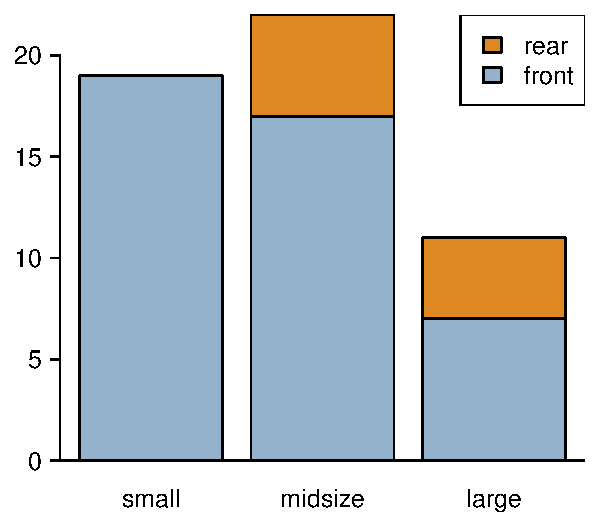
\includegraphics[width=0.46\textwidth]{01/figures/typeDriveTrainSegBarPlot/typeDriveTrainSegBarPlotOrig}
\label{typeDriveTrainSegBarPlotOrig}
}
\subfigure[]{
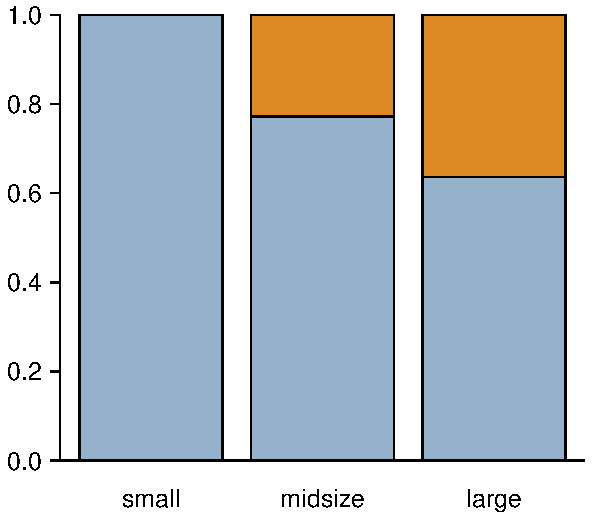
\includegraphics[width=0.46\textwidth]{01/figures/typeDriveTrainSegBarPlot/typeDriveTrainSegBarPlotSta}
\label{typeDriveTrainSegBarPlotSta}
}
\caption{\subref{typeDriveTrainSegBarPlotOrig} Segmented bar plot for vehicle type, where the counts have been broken down by \var{type} then \var{drivetrain}. \subref{typeDriveTrainSegBarPlotSta} Standardized version of Figure~\subref{typeDriveTrainSegBarPlotOrig}.}
\label{typeDriveTrainSegBarPlot}
\end{figure}

The choice to describe each level of \var{drivetrain} within the levels of the \var{type} variable was arbitrary; we could have first created a bar plot of \var{type} and then broken it up using each level of \var{drivetrain}. Just like considering row and column proportions, it is good to evaluate both ways one might construct a segmented bar plot before choosing a final form.

%The left panel of Figure~\ref{typeDriveTrainSegBarPlot} shows a segmented bar plot for the \var{type} variable with a color breakdown to describe the number of vehicles in each group with each type of drive train.

\begin{exercise}
Why is only one level of \var{drivetrain} shown for small vehicles in Figure~\ref{typeDriveTrainSegBarPlot}? %Hint in the footnote\footnote{How many small vehicles have a rear drivetrain?}.
\end{exercise}

%\begin{example}{Figure~\ref{typeDriveTrainSegBarPlotSta} is analogous to Table~\ref{typeDriveTrainTableTotalsMinus4wdMain}(b), where the proportion of vehicles with each drivetrain tends to change from one vehicle type to the next. Can you use this plot to assess whether the two variables appear to be independent?}
%If the variables were independent, then we should observe about the same proportion of front and rear vehicle cars in each type of vehicle in the sample. Instead, there appears to be an association between the two variables since the proportion of each drivetrain appears to change from one vehicle type to another.
%\end{example}

\begin{figure}[p]
\centering
\subfigure[]{
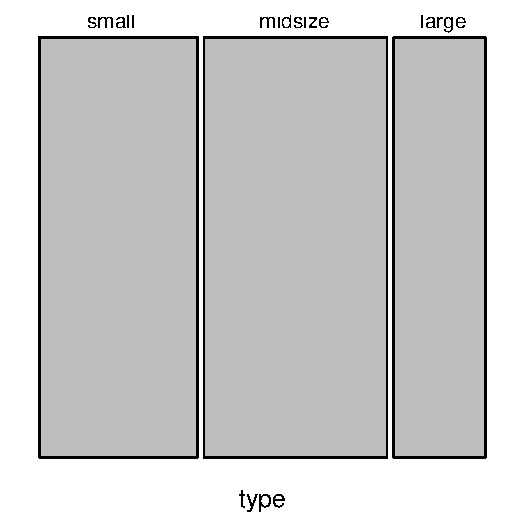
\includegraphics[width=0.46\textwidth]{01/figures/typeDriveTrainMosaicPlot/typeDriveTrainMosaicPlotType}
\label{typeDriveTrainMosaicPlotType}
}
\subfigure[]{
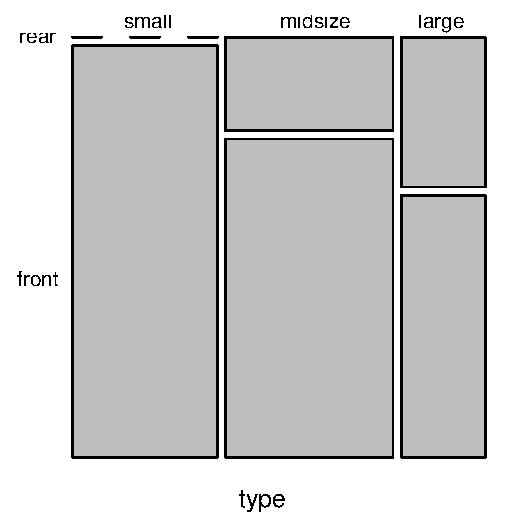
\includegraphics[width=0.46\textwidth]{01/figures/typeDriveTrainMosaicPlot/typeDriveTrainMosaicPlotFull}
\label{typeDriveTrainMosaicPlotFull}
}
\caption{The one-variable mosaic plot for \var{type} and the two-variable mosaic plot for both \var{type} and \var{drivetrain}.}
\label{typeDriveTrainMosaicPlot}
\end{figure}
A \term{mosaic plot} is a graphical display of contingency table information that is similar to a bar plot for one variable or a segmented bar plot when using two variables. 
%Here we construct the mosaic plot representing the row proportions of \var{type} and \var{drivetrain} in Table~\ref{typeDriveTrainTableTotalsMinus4wdMain}(b). 
Figure~\ref{typeDriveTrainMosaicPlotType} shows a mosaic plot for the \var{type} variable from Table~\ref{typeDriveTrainTableTotalsMinus4wdMain}(a). Each column represents a level of \var{type}, and the column widths correspond to the proportion of cars of each type. For instance, there are fewer small cars than midsize cars, so the small car column is slimmer.

This one-variable mosaic plot is further broken into pieces in Figure~\ref{typeDriveTrainMosaicPlotFull} using the \var{drivetrain} variable. Each column is split proportionally according to the drivetrain for vehicles of that particular type. For example, the second column, representing only midsize cars, was broken into midsize cars with front and rear drivetrains. Notice that a dashed line is used to represent small cars with rear wheel drive because there were none. %In the right of Table~\ref{typeDriveTrainTableTotalsMinus4wd}, the proportion of each \var{drivetrain} level was computed within \resp{small}, \resp{midsize}, and \resp{large} cars separately. Similarly, we break apart each of the columns in the left panel of Figure~\ref{typeDriveTrainMosaicPlot} into cars with \resp{front} and \resp{rear} drive trains, which results in the right panel.
As another example, the top of the third column represents large cars with rear wheel drive, and the lower part of the third column represents large cars with front wheel drive. Because each column is broken apart in very different places, this suggests the proportion of vehicles with front wheel drive differs with vehicle \var{type}. That is, \var{drivetrain} and \var{type} show some connection and are therefore associated.
\begin{figure}
   \centering
   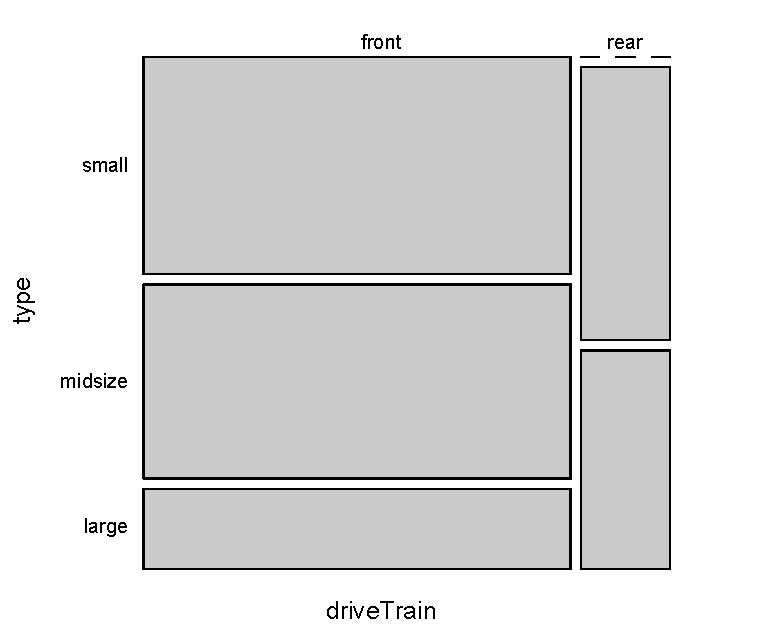
\includegraphics[width=0.65\textwidth]{01/figures/drivetrainTypeMosaicPlot/drivetrainTypeMosaicPlot}
   \caption{Mosaic plot where type is broken up within the drivetrain.}
   \label{drivetrainTypeMosaicPlot}
\end{figure}



In a similar way, a mosaic plot representing column proportions of Table~\ref{typeDriveTrainTableTotalsMinus4wdMain}(a) can be constructed as shown in Figure~\ref{drivetrainTypeMosaicPlot}.

%\begin{exercise}
%What does the mosaic plot on the right of Figure~\ref{typeDriveTrainMosaicPlot} suggest about how a vehicle's \var{type} and \var{drivetrain} are related? Answer in the footnote\footnote{It appears that the larger the vehicle, the more likely it is to have a rear drive train. Do you think this result (that larger vehicles are more likely to have rear drive trains) means a vehicle being larger \emph{causes} the vehicle to have rear wheel drive? This question will be answered in Section~\ref{experiments}.}.
%\end{exercise}

\begin{exercise}
Describe how the mosaic plot shown in Figure~\ref{drivetrainTypeMosaicPlot} was constructed. Answer in the footnote\footnote{First, the cars were split up by \var{drivetrain} into two groups represented by the columns. Then the \var{type} variable splits each of these columns into the levels of \var{type}.}.
\end{exercise}

\subsection{The only pie chart you will see in this book}

While pie charts are well known, they are not typically as useful as other charts in a data analysis. A \term{pie chart} is shown in Figure~\vref{carsTypePieChart} alongside a bar plot. It is more difficult to compare group sizes in a pie chart than in a bar plot. %While pie charts may be helpful in some scenarios, they are not typically as helpful in a strict data analysis setting, which is why this is the first and last pie chart in this book.
\begin{figure}%[bth]
   \centering
   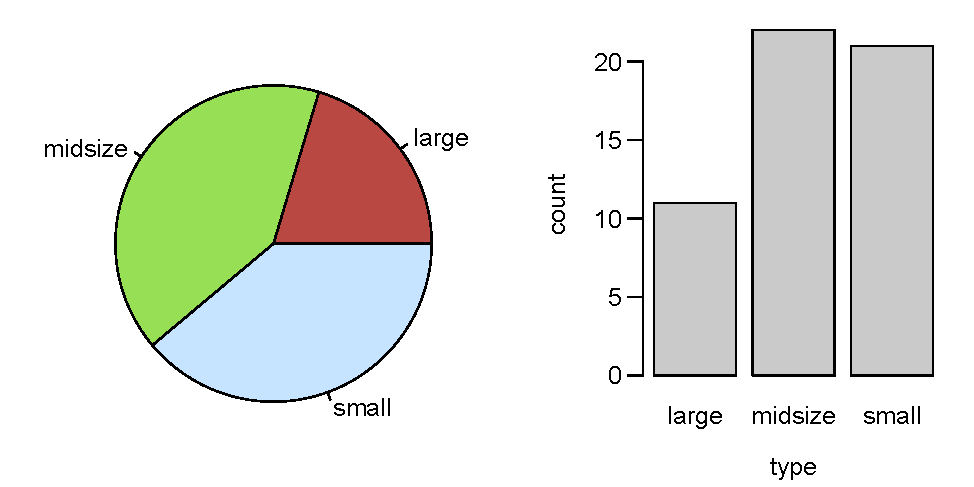
\includegraphics[width=0.8\textwidth]{01/figures/carsTypePieChart/carsTypePieChart}
   \caption{A pie chart and bar plot of \var{type} for the data set \data{cars}.}
   \label{carsTypePieChart}
\end{figure}

\begin{exercise}
Using the pie chart, is it easy to tell which level, \resp{midsize} or \resp{small}, has a larger proportion in the sample? What about when using the bar plot?
\end{exercise}

\subsection{Comparing numerical data across groups}
\label{comparingAcrossGroups}

Some of the more interesting investigations can be considered by examining numerical data across groups. The methods required aren't really new. All that is required is to make a numerical plot for each group. Here two convenient methods are introduced: side-by-side box plots and hollow histograms.

From the data set \data{cars}, we will compare vehicle price according to vehicle type. There are three levels of \var{type} (\resp{small}, \resp{midsize}, and \resp{large}), and the vehicle prices can be split into each of these groups, as shown in Table~\ref{carsPriceSplitByTypeTable}.
\begin{table}
\centering\small
\begin{tabular}{ cc c cc c c }
  \cline{1-2} \cline{4-5}  \cline{7-7}
\multicolumn{2}{c}{\bf small} && \multicolumn{2}{c}{\bf midsize} && {\bf large} \\ 
  \cline{1-2} \cline{4-5}  \cline{7-7}
15900 & 11600 &\hspace{5mm}\ & 33900 & 28000 &\hspace{5mm}\ & 20800 \\ 
9200 & 10300 && 37700 & 35200 && 23700 \\ 
11300 & 11800 && 30000 & 34300 && 34700 \\ 
12200 & 9000 && 15700 & 61900 && 18800 \\ 
7400 & 11100 && 26300 & 14900 && 18400 \\ 
10100 & 8400 && 40100 & 26100 && 29500 \\ 
8400 & 10900 && 15900 & 21500 && 19300 \\ 
12100 & 8600 && 15600 & 16300 && 20900 \\ 
8000 & 9800 && 20200 & 18500 && 36100 \\ 
10000 & 9100 && 13900 & 18200 && 20700 \\ 
8300 &  && 47900 & 26700 && 24400 \\ 
  \cline{1-2} \cline{4-5}  \cline{7-7}
\end{tabular}
\caption{The data from the \var{price} variable split up by \var{type}.}
\label{carsPriceSplitByTypeTable}
\end{table}

The \term{side-by-side box plot} is a traditional tool for comparing across groups. An example is shown in the left panel of Figure~\ref{carsPriceByTypeSBSandHH}, where there are just three box plots -- one for each \var{type} -- placed into one plotting window and drawn on the same scale.
\begin{figure}
   \centering
   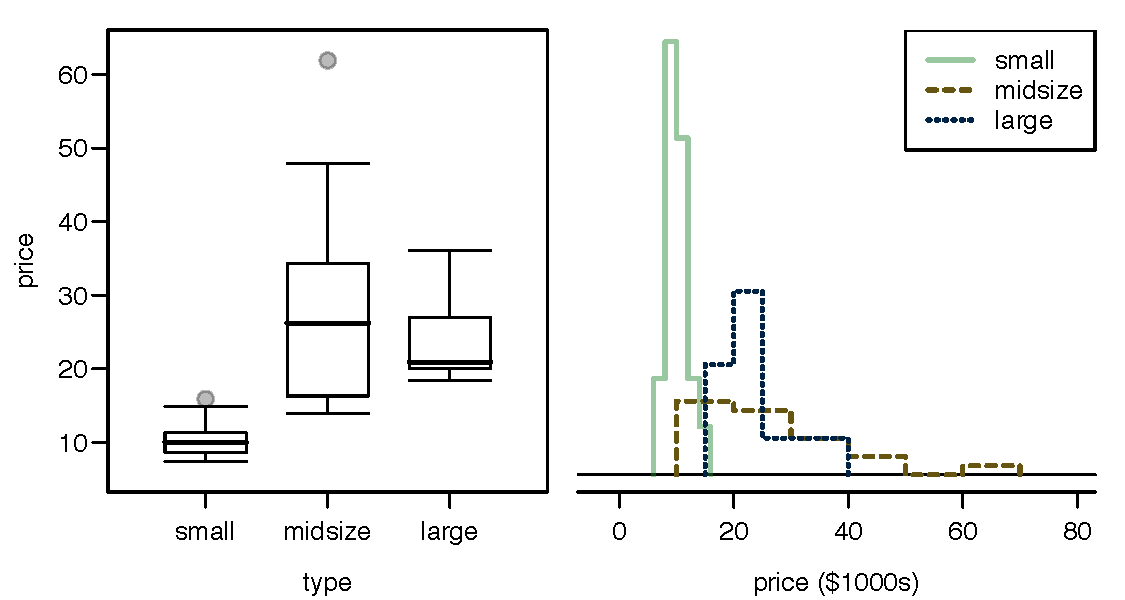
\includegraphics[width=0.85\textwidth]{01/figures/carsPriceByTypeSBSandHH/carsPriceByTypeSBSandHH}
   \caption{Side-by-side box plot (left panel) and hollow histograms (right panel) for \var{price} where the groups represent each level of \var{type}.}
   \label{carsPriceByTypeSBSandHH}
\end{figure}

\termsub{Hollow histograms}{hollow histograms} are another useful plotting method for numerical data. These are just the outlines of histograms of each group put on the same plot, as shown in the right panel of Figure~\ref{carsPriceByTypeSBSandHH}.

\begin{exercise} \label{comparingPriceByTypeExercise}
Use each plot in Figure~\ref{carsPriceByTypeSBSandHH} to compare the vehicle prices across groups. What do you notice about the approximate center of each group? What do you notice about the variability between groups? Is the shape relatively consistent between groups? How many \emph{prominent} modes are there for each group?
\end{exercise}

\begin{exercise}
What components of each plot in Figure~\ref{carsPriceByTypeSBSandHH} do you find most useful?
\end{exercise}


%%%%%
\section{Overview of data collection principles}
\label{overviewOfDataCollectionPrinciples}

The first step in conducting research is to identify topics or questions that are to be investigated. A clearly laid out research question is helpful in identifying what subjects or cases are to be studied and what variables are important. This information provides a foundation for \emph{what} data will be helpful. It is also important that we consider \emph{how} data are collected so that they are trustworthy and help achieve the research goals. %Researchers can be actively engaged in studies called experiments, or they can observe behaviors and collect data in a more passive framework through observational studies. We consider observational studies and data collection methods in this section and then address experiments in Section~\ref{experimentsSection}.

\subsection{Populations and samples}
\label{populationsAndSamples}

Consider the following three research questions:
\begin{enumerate}
\setlength{\itemsep}{0mm}
\item What is the average mercury content in swordfish in the Atlantic Ocean?
\item\label{timeToGraduationQuestionForUCLAStudents} Over the last 5 years, what is the average time to degree for UCLA undergraduate students?
\item\label{identifyPopulationOfSulphinpyrazone} Does the drug sulphinpyrazone reduce the number of deaths in heart attack patients?
\end{enumerate}
In each research question, some population of cases is considered. In the first question, all swordfish in the Atlantic ocean are relevant to answering the question. Each fish represents a case, and all of these fish represent the \term{population} of cases. Often times, it is too expensive to collect data for every case in a population. Instead a sample is taken. A \term{sample} represents a subset of the cases and is often a small fraction of the population. For instance, 60 swordfish (or some other number) in the population might be selected, and this sample data may be used to provide an estimate of the population average, i.e. an answer to the research question.

\begin{exercise} \label{identifyingThePopulationForTwoQuestionsInPopAndSampSubsection}
For the second and third questions above, identify what is an individual case and also the population under consideration. Answers in the footnote\footnote{(\ref{timeToGraduationQuestionForUCLAStudents}) First, notice that this question is only relevant to students who complete their degree; the average cannot be computed using a student who never finished her degree. Thus, only UCLA undergraduate students who have graduated in the last five years represent cases in the population under consideration. (\ref{identifyPopulationOfSulphinpyrazone}) A heart attack patient represents a case. The population represents all heart attack patients.}.
\end{exercise}


\subsection{Anecdotal evidence}

Consider the following possible responses to our three research questions:
\begin{enumerate}
\item A man on the news got mercury poisoning from eating swordfish, so the average mercury concentration in swordfish must be dangerously high.
\item\label{iKnowThreeStudentsWhoTookMoreThan10YearsToGraduateAtUCLA} I met two students who took more than 10 years to graduate from UCLA, so it must take longer to graduate at UCLA than at many other colleges.
\item\label{myFriendsDadDiedAfterSulphinpyrazon} My friend's dad had a heart attack and died after they gave him sulphinpyrazone. The drug must not work.
\end{enumerate}
Each of the conclusions are based on some data. However, there are two problems. First, the data only represent one or two cases. Second and more importantly, it is unclear whether these cases are actually representative of the population. Data collected in this haphazard fashion are called \term{anecdotal evidence}.
\setlength{\captionwidth}{\textwidth-64mm}
\begin{figure}
\begin{centering}
\includegraphics[width=55mm]{01/figures/mnWinter/mnWinter}\hspace{4mm}
\begin{minipage}[b]{\textwidth - 64mm}
   \caption[anecdotal evidence]{In February 2010, some media pundits cited one large snow storm as valid evidence against global warming. As comedian Jon Stewart pointed out, ``It's one storm, in one region, of one country.''\vspace{-4.5mm} \\
   
   -----------------------------\vspace{-2mm}\\
   {\footnotesize February 10th, 2010.}
   \label{mnWinter}}
\end{minipage}
\end{centering}
\end{figure}
\setlength{\captionwidth}{\mycaptionwidth}

\begin{termBox}{\tBoxTitle{Anecdotal evidence}
Data collected in a haphazard fashion. Such evidence may be true and verifiable but often times represents extraordinary cases.}
\end{termBox}

Anecdotal evidence typically is composed of unusual cases that we recall based on their striking characteristics. For instance, we are more likely to remember the two folks we met who took 10 years to graduate than the six others who graduated in four years. Instead of looking at the most unusual cases, we should examine a sample of many cases that represent the population.

\subsection{Sampling from a population}

The \data{cars} data set represents a {sample} of cars from 1993. All cars from 1993 represent the {population}, and the cars in the sample were \emph{randomly} selected from the population. Random selection in this context is equivalent to how raffles are run. The name of each car from the population was written on a raffle ticket, and 54 tickets were drawn.
\begin{figure}[ht]
\centering
\includegraphics[height=1.5in]{01/figures/popToSample/popToSample}
\caption{Cars from the population are randomly selected to be included in the sample.}
\label{popToSample}
\end{figure}

Why pick a sample randomly? Why not just pick a sample by hand? Consider the following scenario.

\begin{exercise}
Suppose a muscle car enthusiast is asked to select several cars for a study. What kind of cars do you think she might collect? Do you think her sample would be representative of all cars?
\end{exercise}
\begin{figure}
\centering
\includegraphics[height=1.5in]{01/figures/popToSample/popToSubSample}
\caption{Instead of sampling from all cars from 1993, an environmentalist might inadvertently pick cars with high mileage disproportionally often.}
\label{popToSubSample}
\end{figure}

If someone was permitted to pick and choose exactly which cars were included in the sample, it is entirely possible that the sample could be skewed to that person's interests, which may be entirely unintentional. This introduces \term{bias} into a sample. Sampling randomly helps resolve this problem. The most basic random sample is called a \term{simple random sample}, and is the equivalent of using a raffle to select cases. This means that each case in the population has an equal chance of being included and there is no implied connection between the cases in the sample. The act of taking a simple random sample helps eliminate bias, however, bias can still crop up in other ways.

Even when people are seemingly picked at random (for surveys, etc.), caution must be exercised if the \term{non-response} is high. For instance, if only 15\% of the people randomly sampled for a survey actually respond, then it is unclear whether the results are \term{representative} of the entire population. This \term{non-response bias} can skew results.
\begin{figure}[h]
\centering
\includegraphics[height=1.5in]{01/figures/popToSample/surveySample}
\caption{Surveys may result in only reaching a certain group within the population, and it is not obvious how to fix this problem.}
\label{surveySample}
\end{figure}

Another common downfall is a \term{convenience sample}, where individuals who are easily accessible are more likely to be included in the sample. For instance, if a political survey is done by stopping people walking in the Bronx, this probably will not fairly represent all of New York City. It is often difficult to discern what sub-population a convenience sample represents.

\begin{exercise}
We can easily access ratings for products, sellers, and companies through websites. These ratings are based only on those people who go out of their way to provide a rating. If a seller has a rating of 95\% on Amazon, do you think this number might be artificially low or high? Why?
\end{exercise}

\subsection{Explanatory and response variables}
\label{explanatoryAndResponse}

Consider the second question from page~\pageref{possibleCausationQuestionForPossums} for the \data{possum} data set:
\begin{enumerate}
\item[(2)] Will males or females, on the average, be longer?
\end{enumerate}
This question might stem from the belief that a possum's gender might in some way affect its size. If we suspect a possum's sex might affect its total length, then \var{sex} is the \term{explanatory} variable and \var{totalL} is the \term{response} variable in the relationship\footnote{Sometimes the explanatory variable is called the \term{independent} variable and the response variable is called the \term{dependent} variable. However, this becomes confusing since a \emph{pair} of variables might be independent or dependent, so we avoid this language.}. If there are many variables, it may be possible to label a number of them as explanatory and the others as response variables.

\begin{tipBox}{\tipBoxTitle{Explanatory and response variables}
To identify the explanatory variable in a pair of variables, identify which of the two is suspected of affecting the other.

\hspace{10mm}\includegraphics[height=0.34in]{01/figures/expResp/expResp}}
\end{tipBox}

\begin{caution}{association does not imply causation}{Labeling variables as \emph{explanatory} and \emph{response} does not guarantee the relationship between the two is actually causal, even if there is an association identified between the two variables. We use these labels only to keep track of which variable we suspect affects the other.}
\end{caution}

In some cases, there is no explanatory or response variable. Consider the first question from page~\pageref{possumHeadSizeQuestion}:
\begin{enumerate}
\item[(1)] If a possum has a shorter-than-average head, do you think its skull width will be smaller or larger than the average skull width?
\end{enumerate}
This question does not have an explanatory variable since it is unclear whether \var{headL} would affect \var{skullW} or vice-versa, i.e. the direction is ambiguous.

\subsection{Introducing observational studies and experiments}

There are two primary types of data collection: observational studies and experiments.

Researchers perform an \term{observational study} when they collect data in a way that does not directly interfere with how the data arise. For instance, researchers may collect information using surveys, reviewing medical or company records, or follow a \term{cohort} of many similar individuals to consider why certain diseases might develop. In each of these cases, the researchers try not to interfere with the natural order of how the data arise. In general, observational studies can provide evidence of a naturally occurring association between variables, but they cannot show a causal connection.

When researchers want to establish a causal connection, they conduct an \term{experiment}. Usually there will be both an explanatory and a response variable. For instance, we may suspect administering a drug will reduce mortality in heart attack patients over the following year. To check if there really is a causal connection between the explanatory variable and the response, researchers will collect a sample of individuals and split the cases into groups. The cases in each group are \emph{assigned} a treatment. When the groups are created using a randomization technique, the experiment is called a \term{randomized experiment}. For example, each heart attack patient in the drug trial could be randomly assigned (e.g. by flipping a coin) into one of two groups: the first group receives a placebo (fake treatment) and the second group receives the drug.

\begin{tipBox}{\tipBoxTitle{association $\neq$ causation}
In general, association does not imply causation, and causation can only be inferred from a randomized experiment.}
\end{tipBox}


%%%%%
\section{Observational studies and sampling strategies}

\subsection{Observational studies}

The \data{possum} data set was from an observational study. While researchers captured the possums, their measurements and other variables were naturally occurring. Generally, data in observational studies are collected only by monitoring what occurs, while experiments require the primary explanatory variable in a study be assigned for each subject by the researchers.

Inferring causal conclusions from experiments is often reasonable. However, making the same causal conclusions from observational data can be treacherous and is not recommended. Thus, we can generally only infer associations from observational data.

\begin{exercise} \label{sunscreenLurkingExample}
Suppose an observational study tracked sunscreen use and skin cancer, and it was found that the more sunscreen someone used, the more likely the person was to have skin cancer. Does this mean sunscreen \emph{causes} skin cancer?
\end{exercise}

Previous research tells us that using sunscreen actually reduces skin cancer risk, so maybe there is another variable that can explain this hypothetical association between sunscreen usage and skin cancer. One important piece of information absent is sun exposure. If someone is out in the sun all day, she is more likely to use sunscreen \emph{and} more likely to get skin cancer.
\begin{center}
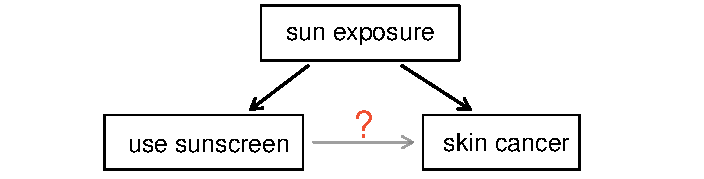
\includegraphics[height=1.0in]{01/figures/variables/sunCausesCancer}
\end{center}
It just so happens that if someone is exposed to the sun they also usually use sunscreen. Exposure to the sun is unaccounted for in the investigation, giving the incorrect impression that sunscreen causes skin cancer.

Sun exposure is what is called a \term{lurking variable}\footnote{Also called a \term{confounding variable}, \term{confounding factor}, or a \term{confounder}.}, which is a variable that is correlated with both the explanatory and response variables. While one method to justify making causal conclusions from observational studies is to exhaust the search for lurking variables, there is no guarantee that all lurking variables can be examined or measured.

In the same way, the \data{possum} data set is an observational study with possible lurking variables of its own, and its data cannot easily be used to make causal conclusions.

\begin{exercise}
There appears to be a real difference in the proportion of possums that are male based on location. However, it is unreasonable to conclude that this is a causal relationship because the data are observational. Suggest at least one lurking variable that might be the true cause for the differences in \var{sex}. One possibility is listed in the footnote\footnote{Some genes can affect one gender more than the other. If the \resp{other} population has a gene that affects males more positively than females and this gene is less common in the \resp{Vic} population, this might explain the difference in gender ratio for each level of \var{pop}.}.
\end{exercise}

Observational studies come in two forms: prospective and retrospective studies. A \term{prospective study} identifies individuals and collects information as events unfold. For instance, medical researchers may identify and follow a group of similar individuals over many years to assess the possible influences of behavior on cancer risk. \termsub{Retrospective studies}{retrospective studies} collect data after events have taken place, e.g. researchers may review past events in medical records. The \data{possum} data are an example of a retrospective study.

\subsection{Three sampling methods (special topic)}
\label{threeSamplingMethods}

Almost all statistical methods are based on the notion of implied randomness. If observational data are not collected in a random framework from a population, these statistical methods -- the estimates and computed errors -- are not reliable. Here we consider three random sampling techniques: simple, stratified, and cluster sampling. We introduce these techniques in the context of Major League Baseball (MLB) salary data, where each player is a member of one of the league's 30 teams, and we consider taking a sample of 120 players.

\emph{Simple random sampling} is probably the most intuitive form of random sampling. To take a simple random sample of the baseball players and their salaries, we could write each player's name on a ping pong ball, drop the ping pong balls into a bucket, shake the bucket around until we are sure it's all mixed up, then draw out balls from the bucket until we have the sample of 120 players. In general, a sample is referred to as ``simple random'' if each case in the population has an equal chance of being included in the final sample \emph{and} knowing that a case is included in a sample does not provide useful information about which other cases/outcomes are included.

\termsub{Stratified sampling}{stratified sampling} is a divide-and-conquer sampling strategy. The population is divided up into groups called \term{strata} where the strata are chosen so that similar cases are grouped, then a second sampling method (such as simple random sampling) is employed within each stratum. In the baseball salary example, the teams could represent the strata; some teams have much more money (we're looking at you, Yankees). Then we might randomly sample four players from each team for a total of 120 players.

Stratified sampling is especially useful when the cases in each stratum are very similar in the measured outcome. For instance, the baseball teams might be useful strata since some teams have (much) more money and therefore tend to pay players more. The downside is that analyzing data from a stratified sample is more complex than analyzing data from a simple random sample, and the analysis methods introduced in this book would need to be extended.

\begin{example}{Why would it be good for cases within each stratum to be very similar?}
We might get a more stable statistical estimate for the subpopulation in a stratum if the cases are very similar. Then when we summarize the entire population, these individual stable estimates for each subpopulation will help us build a reliable estimate for the full population.
\end{example}

A \term{cluster sample} is much like a two-stage simple random sample. We break up the population into many groups, called \term{clusters}. Then we sample a fixed number of clusters and collect a simple random sample in each cluster. This technique is very similar to stratified sampling in its process, except that there is no requirement to sample from every cluster while stratified sampling requires observations from every stratum.
\begin{figure}
\centering
\includegraphics[width=0.8\textwidth]{01/figures/samplingMethodsFigure/samplingMethodsFigure}
\caption{Examples of simple random, stratified, and cluster sampling. In the top panel, simple random sampling was used to randomly select the 18 cases. In the middle panel, stratified sampling was used: cases were grouped into strata, and then simple random sampling was employed within each stratum. In the bottom panel, cluster sampling was used, where data were binned into nine clusters, three of the clusters were randomly selected, and six cases were randomly sampled in each of these clusters.}
\label{samplingMethodsFigure}
\end{figure}

Sometimes cluster sampling can be a more economical random sampling technique than alternatives. Also, unlike stratified sampling, cluster sampling is most helpful when there is a lot of case-to-case variability within a cluster but the clusters themselves don't look very different from one another (e.g. if neighborhoods represented clusters, then it is best if each neighborhood is very diverse). A downside of cluster sampling is that more advanced analysis techniques are typically required, though the methods in this book can be extended to handle such data.

\begin{example}{Describe a scenario where cluster sampling would be much easier than simple random or stratified sampling.}
Suppose we are interested in estimating the malaria rate in a densely tropical portion of rural Indonesia. We believe there are 30 villages in that part of the Indonesian jungle, each more or less similar to the next. Our goal is to test 150 individuals for malaria. In this case, a simple random sample would likely draw individuals from all 30 villages, which could make data collection extremely expensive. Stratified sampling would be a challenge since it is unclear how we would build stratum of similar individuals. However, cluster sampling seems like a very good idea. First, we might randomly select half the villages, then randomly select 10 people from each. This would probably reduce our data collection costs substantially in comparison to a simple random sample and would still give us reliable information.

%Suppose we were sampling tree circumferences in a large forest. It is unclear how we might randomly sample individual trees -- and even if we could, it would be a substantial trek to reach each individual tree in the sample. While it seems possible to build up strata, perhaps using regions in the forest, it is still unclear how we should sample the trees in each stratum. If there are only a small number of strata, we run into the same trouble as in simple random sampling. Additionally, the strata are probably not terribly uniform; tree sizes often vary quite a bit, even in a small region.  If there are many strata, then we must travel far and wide to reach each of them.

%A cluster sample would be much easier to employ, and there are a number of possible cluster sampling strategies -- we present one. We could first divide up the forest into a grid of squares that are 10 meters on each side\footnote{One possible objection: we also must be able to find the precise locations in the forest when we collect data. However, a GPS device could resolve this concern.}. Each of these grid regions could represent a cluster. Next we could randomly sample the clusters where we would actually take tree measurements. For each selected cluster, we might just conduct an exhaustive sample, measuring the circumference of all the trees in that cluster.
\end{example}

\begin{exercise}
Describe a second situation where cluster sampling would be more convenient than simple random or stratified sampling.
\end{exercise}

%The three sampling techniques are depicted in Figure~\ref{samplingMethodsFigure}. Cases are seemingly pulled at random in the top panel, representing simple random sampling. In the middle panel, the data are divided into strata, then we take a random sample of three cases per strata. Cluster sampling is represented in the bottom panel, where the data were divided into many clusters, three of these clusters were randomly selected for sampling, and then six cases were randomly selected in each cluster.


%%%%%
\section{Experiments}
\label{experimentsSection}

Studies where the researchers assign treatments to cases are called \term{experiments}. When cases are randomly assigned to the treatment groups, it is called a \term{randomized experiment}. Randomized experiments are fundamentally important when trying to show a causal connection between two variables.

\subsection{Principles of experimental design}
\label{experimentalDesignPrinciples}

Randomized experiments are generally built on four principles.
\begin{description}
\item[Controlling.] Researchers assign treatments to cases, and they do their best to \term{control} any other differences in the groups. For instance, if a drug treatment in the form of a pill may be affected by how much water a patient drinks with the drug, the doctor may ask all patients to drink a 12 ounce glass of water with the pill to reduce one source of unnecessary variability between the cases.
\item[Randomization.] Researchers randomize patients into the groups to account for variables that cannot be controlled. In a clinical trial, some patients may be more susceptible to a disease than others due to their genetic make-up. Randomizing patients into the two treatment groups is one way to help even out the genetic differences in each group, and it also prevents accidental bias from entering the study.
\item[Replication.] The more cases researchers observe, the more accurately they can estimate the effect of the explanatory variable on the response. In a single study, we \term{replicate} by collecting a sufficiently large sample. Additionally, a group of scientists may replicate an entire study to verify an earlier finding.
\begin{figure}
\centering
\includegraphics[width=0.78\textwidth]{01/figures/figureShowingBlocking/figureShowingBlocking}
\caption{Blocking using a variable depicting patient risk. Patients are first divided into low-risk and high-risk blocks, then each block is evenly divided into the treatment groups using randomization. This strategy ensures an equal number of patients in each treatment group from both the low-risk and high-risk categories.}
\label{figureShowingBlocking}
\end{figure}
\item[Blocking.] Researchers sometimes know or suspect variables other than the treatment that might influence the response. Under this circumstance, they may first group individuals based on this variable into \term{blocks} and then randomize cases within each block to the treatment groups. This strategy is often referred to as \term{blocking}. For instance, if we were looking at the effect of a drug on heart attacks, we might first split patients in the study into low-risk and high-risk blocks, then randomly assigning half the patients from each block to the control group and the other half to the treatment group, as shown in Figure~\ref{figureShowingBlocking}. This strategy ensures each treatment group has an equal number of low-risk and high-risk patients.
\end{description}

It is important to incorporate the first three experimental design principles into any study, and this book describes applicable methods for analyzing data from such experiments. Blocking is a slightly more advanced technique, and statistical methods in this book may be extended to analyze data collected using blocking.

\subsection{Reducing bias in human experiments}
\label{biasInHumanExperiments}

Randomized experiments are the gold standard for data collection, but they do not ensure an unbiased perspective into the cause and effect relationships in all cases. Human studies are perfect examples where bias can unintentionally arise. Here we reconsider the sulphinpyrazone study described in Section~\ref{basicExampleOfSulphinpyrazone}.

Researchers wanted to examine whether a drug called sulphinpyrazone would reduce the number of deaths after heart attacks. They designed a randomized experiment because they wanted to draw causal conclusions about the drug's effect. Study volunteers\footnote{Human subjects are more often called \term{patients}, \term{volunteers}, or \term{study participants}.} were randomly placed into two study groups. One group, the \term{treatment group}, received the drug. The other group, called the \term{control group}, did not receive any drug treatment.

Put yourself in the place of a person in the study. If you are in the treatment group, you are given a fancy new drug that you anticipate will help you. On the other hand, a person in the other group doesn't receive the drug and sits idly, hoping her participation doesn't increase her risk of death. These perspectives suggest there are actually two effects: the one of interest is the effectiveness of the drug and the second is an emotional effect that is difficult to quantify.

Researchers aren't interested in this emotional effect, which might bias the study. To circumvent this problem, researchers do not want patients to know which group they are in. When researchers keep the patients uninformed about their treatment, the study is said to be \term{blind}. But there is one problem: if a patient doesn't receive a treatment, she will know she is in the control group. The solution to this problem is to give fake treatments to patients in the control group. A fake treatment is called a \term{placebo}, and an effective placebo is the key to making a study truly blind. A classic example of a placebo is a sugar pill that is made to look like the actual treatment pill. Often times, a placebo results in a slight but real improvement in patients. This often positive effect has been dubbed the \term{placebo effect}.

The patients are not the only ones who should be blinded: doctors and researchers can accidentally bias a study. When a doctor knows a patient has been given the real treatment, she might inadvertently give that patient more attention or care than a patient that she knows is on the placebo. To guard against this bias (which again has been found to have a measurable effect in some instances), most modern studies employ a \term{double-blind} setup where doctors or researchers who interact with patients are, just like the patients, unaware of who is or is not receiving the treatment\footnote{There are always some researchers involved in the study who do know which patients are receiving which treatment. However, they do not have interactions with the patients and do not tell the blinded doctors who is receiving which treatment.}.

\section{Case study: efficacy of sulphinpyrazone (special topic)}
\label{caseStudyOfSulphinpyrazone}

%An asterisk (*) attached to a section means that section is optional. To utilize this optional section, it is recommended that an accompanying lab using these same methods on a second data set is incorporated into the class.

%In this section, we examine a case study. In Chapter~\ref{foundationsForInference}, we will revisit these topics in greater detail

\begin{example}{Suppose your professor splits the students in class into two groups: students on the left and students on the right. If $\hat{p}_{_L}$ and $\hat{p}_{_R}$ represent the proportion of students who own an Apple product on the left and right, respectively, would you be surprised if $\hat{p}_{_L}$ did not {exactly} equal $\hat{p}_{_R}$?}\label{classRightLeftSideForHeight}
While the proportions would probably be close to each other, it would be unusual for them to be exactly the same. We would probably observe a small difference due to {chance}.
\end{example}

\begin{exercise}
If we don't think the side of the room a person sits on in class is related to whether the person owns an Apple product, what assumption are we making about the relationship between the \var{sideOfRoom} and \var{ownsAppleProduct} variables? %How might we check this assumption? 
Answer in the footnote\footnote{We would be assuming the variables \var{sideOfRoom} and \var{ownsAppleProduct} are independent. %To evaluate the assumption, we could collect data. If we find that the proportion of students on one side of the room who own an apple product is very different than the proportion on the other side, we could view this as convincing evidence that our assumption is wrong. (Note: the difference being approximately equal doesn't mean we are right. If the number of students on either side is about the same, then it might just suggest the variables are \emph{nearly} independent.) 
}.
\end{exercise}

\subsection{Variability within data}
\label{variabilityWithinData}

The study examining the effect of sulphinpyrazone introduced in Section~\ref{basicExampleOfSulphinpyrazone} was double-blinded, and the results are summarized in Table~\ref{sulphinpyrazoneResults}. The variables have been called \var{group} and \var{outcome}. Do these results mean the drug was effective at reducing deaths? In the observed groups, a smaller proportion of individuals died in the treatment group than the control group (0.056 versus 0.081), however, it is unclear whether that difference represents \emph{convincing evidence} that the drug is effective.
\begin{table}[ht]
\centering
\begin{tabular}{l l cc rr}
& & \multicolumn{2}{c}{\var{outcome}} \\
  \cline{3-4}
		&			& 	\resp{lived} 	& \resp{died} & Total & \hspace{3mm}  \\ 
  \cline{2-5}
		&	\resp{treatment} 	& 692    		& 41   & 733  	 \\ 
  \raisebox{1.5ex}[0pt]{\var{group}}		&	\resp{control} 	& 682    		& 60     & 742	 \\ 
  \cline{2-5}
  		&	Total		& 1374	& 101	&  1475 \\
  \cline{2-5}
\end{tabular}
\vspace{-2mm}
\caption{Summary results for the sulphinpyrazone study.}
\label{sulphinpyrazoneResults}
\end{table}

\begin{example}{Statisticians are sometimes called upon to evaluate the strength of evidence. When looking at the death rates in the study, what comes to mind as we try to determine whether the data show convincing evidence of a real difference?} \label{sulphinpyrazoneResultsWhatIsConvincingEvidence}
The observed death rates (0.056 versus 0.081) suggest the drug may be effective since the treatment group has a lower proportion of deaths. However, the sample proportions are very close. Generally there is a little bit of fluctuation in sample data, and we wouldn't expect the sample proportions to be \emph{exactly} equal even if the truth was that they were equal across the two treatments. As we look at the data, we want to ask, is the difference between the death rates so large that it probably isn't due to chance?
\end{example}

%\begin{example}{Suppose there had been only 45 deaths in the control group and still only 41 deaths in the treatment group. Would this be convincing evidence that the drug was effective?} \label{45PlaceboDeaths}
%At this stage in our statistical development, it is difficult to stay. These proportions still favor the drug's effectiveness (0.056 death rate versus 0.061), but the proportions are very close. Generally there is a little bit of wiggle in sample data, and we wouldn't expect the proportions to be \emph{exactly} equal. However, if the truth is that the ``true'' death rates are equal, we also would not expect the differences in the proportions to be very big, and larger differences tend to provide stronger evidence of a real difference. In statistics constitutes \emph{convincing evidence}, also called \term{statistical significance}, depends on how much wiggle we would expect from random fluctuations.
%\end{example}

Example~\exam{sulphinpyrazoneResultsWhatIsConvincingEvidence} is a reminder that the sample will not perfectly reflect the population. It is possible to see a small difference by chance. Small differences in large samples can be important and meaningful but it is unclear when we should say that a difference is so large it was probably not due to chance. %In Section~\ref{caseStudyOfSulphinpyrazone}, we evaluate whether Table~\ref{sulphinpyrazoneResults} shows convincing evidence that sulphinpyrazone is effective at reducing deaths or whether we remain unconvinced.
Table~\ref{sulphinpyrazoneResults} shows there were 19 fewer deaths in the treatment group than in the control group for the sulphinpyrazone study, a difference in death rates of 2.5\% $\left( \frac{60}{742} - \frac{41}{733} = 0.025 \right)$. %Is it plausible that this difference is due to chance and the drug actually had no effect on the patient outcome? Or i
Might this difference just be due to chance? Or is this convincing evidence that sulphinpyrazone works? We label these two competing claims, $H_0$ and $H_A$:
\begin{itemize}
\setlength{\itemsep}{0mm}
\item[$H_0$:] \textbf{Independence model.} The variables \var{group} and \var{outcome} are independent. They have no relationship, and the difference in death rates, 2.5\%, was due to chance.
\item[$H_A$:] \textbf{Alternative model.} The \var{group} and \var{outcome} variables are \emph{not} independent. The difference in death rates of 2.5\% was not due to chance and the treatment did reduce the death rate.
\end{itemize}

%In Example~\exam{classRightLeftSideForHeight}, it was acknowledged that the mean heights of two groups will be about the same, however, they are rarely \emph{exactly} the same. The important question for the sylphinpyrazone study is, Is the difference 19 so large that it does not seem reasonable for the variables to be independent?

Consider what it would mean to the study if the independence model, which says that the variables \var{group} and \var{outcome} are unrelated, is true. Each person was either going to live or die, and the drug had no effect on the outcome. The researchers were just randomly splitting up these individuals into two groups, very much like we split the class in half in Example~\exam{classRightLeftSideForHeight}. The researchers observed a difference of 2.5\% by chance.

Consider the alternative: the treatment affected the outcome. We would expect to see some difference in the groups, with a lower percentage of deaths in the group of patients who received the drug.

If the data conflict so much with $H_0$ that the independence model cannot be deemed reasonable, we will reject it in favor the alternative model, $H_A$. In other words, we will not reject the position that $H_0$ is true unless the evidence from the study in favor of $H_A$ is extremely convincing.

\subsection{Simulating the study}

Suppose $H_0$ is true. Under this model, the 2.5\% difference would have been due to chance, and the group assignments would not have impacted the patient outcomes. We will use this thought experiment to simulate differences that are due to chance using a \term{randomization technique}.

We are going to recreate (simulate) the study under the scenario that patient outcome has nothing to do with the treatment. To do this, we are going to randomly reassign the patients into a fake treatment or fake control group. Then, since we know this fake group assignment has nothing to do with the patients' actual outcomes -- the fake group assignment and the outcome are independent -- any observed difference in death rates between the fake groups must be due to chance.

We run this \term{simulation} by taking 733 \resp{treatmentFake} and 742 \resp{controlFake} labels and randomly assign them to the patients. These label counts correspond to the number of \var{treatment} and \var{control} assignments in the actual study. We use a computer program to randomly assign these labels to the patients, and we organize these results into Table~\ref{sulphinpyrazoneRand1}.
\begin{table}[ht]
\centering
\begin{tabular}{l l cc rr}
& & \multicolumn{2}{c}{\var{outcome}} \\
  \cline{3-4}
		&			& 	\resp{lived} 	& \resp{died} & Total & \hspace{3mm}  \\ 
  \cline{2-5}
		&	\resp{treatmentFake} 					& 686    		& 47    & 733 	 \\ 
  \raisebox{1.5ex}[0pt]{\var{groupFake}}		&	\resp{controlFake} 	& 688    		& 54 & 742    	 \\ 
  \cline{2-5}
\end{tabular}
\caption{Simulation results, where any difference in death rates between \resp{treatmentFake} and \resp{controlFake} is purely due to chance.}
\label{sulphinpyrazoneRand1}
\end{table}

%Running this simulation many times, we get an idea for what represents common differences under the independence model, and we can evaluate whether the observed difference, 2.5\%, is too big to plausibly be due to chance.
%\begin{center}
%Independence model \\
%$\downarrow$ \\
%differences due to chance
%\end{center}
%If 2.5\% is an uncommonly large difference from the independence model, then we would conclude that this model does not fit our data and we reject $H_0$ in favor of $H_A$, that the drug is actually effective.

\begin{exercise} \label{sampleDifferenceInDrugAndPlaceboGroupSulph}
What is the difference in death rates between the two fake groups in Table~\ref{sulphinpyrazoneRand1}? How does this compare to the observed 2.5\% in the real groups? Answer in the footnote\footnote{$54/742 - 47/733=0.0087$ or about 0.9\%. This difference due to chance is smaller.}. % However, we should run more simulations to get a good idea of what differences we get by chance, i.e. it is possible 0.9\% was a fluke.}.
\end{exercise}

\subsection{Checking for independence}

We computed one possible difference under the independence model in Exercise~\exer{sampleDifferenceInDrugAndPlaceboGroupSulph}, which represents one difference due to chance. We could repeat the simulation to get another difference from chance: -0.005. And another: -0.010. And another: 0.003. And so on until we repeat the simulation enough times that we have a good idea of what represents the \emph{distribution of differences from chance alone}. Figure~\ref{sulphRandHist} shows a histogram of the differences found from 100 simulations.
\setlength{\captionwidth}{\mycaptionwidth+3mm}
 \begin{figure}[ht]
    \centering
    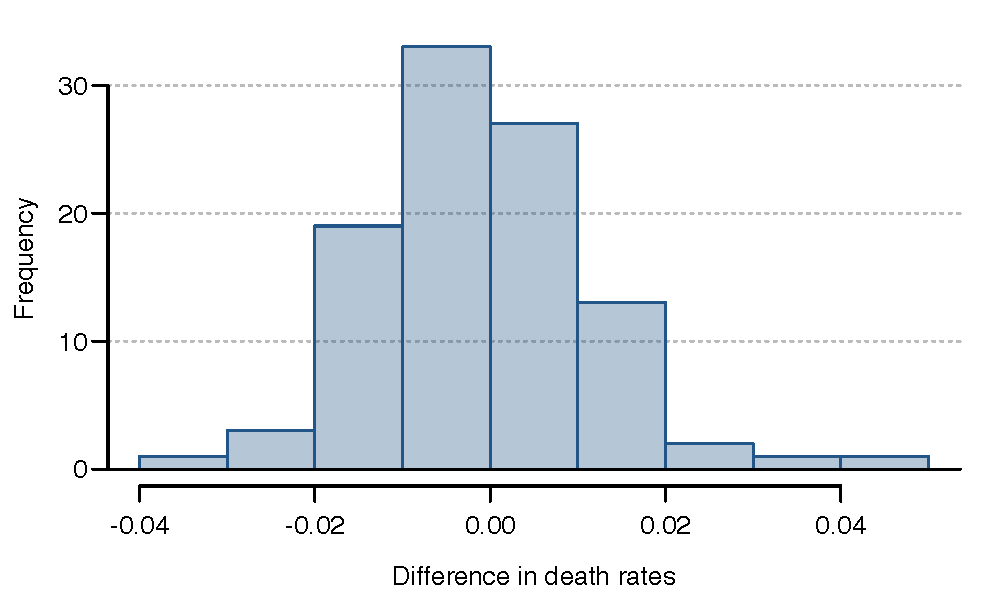
\includegraphics[width=0.7\textwidth]{01/figures/sulphRandHist/sulphRandHist}
    \caption{A histogram of differences from 100 simulations produced under the independence model, $H_0$, where \var{groupFake} and \var{outcome} are independent. Four of the one-hundred simulations had a difference of at least 2.5\%.}
    \label{sulphRandHist}
 \end{figure}
\setlength{\captionwidth}{\mycaptionwidth}
 
\begin{example}{How often would you observe a difference of 2.5\% (0.025) according to Figure~\ref{sulphRandHist}? Often, sometimes, rarely, or never?}
It appears that a difference of at least 2.5\% due to chance alone would only happen about 4\% of the time according to Figure~\ref{sulphRandHist}. We might describe that as being a rare event.
\end{example}

The difference of 2.5\% is a rare event, and this suggests two possible interpretations of the results of the study:
\begin{itemize}
\setlength{\itemsep}{0mm}
\item[$H_0$] \textbf{Independence model.} The drug doesn't work, and we observed a difference that would only happen rarely.
\item[$H_A$] \textbf{Alternative model.} The drug does work, and what we observed was that the drug was actually working, which explains the large difference of 2.5\%.
\end{itemize}
We should be skeptical that what was observed just happened to be a rare event, and we usually reject the null hypothesis in a situation like this and conclude the drug works.

One field of statistics, statistical inference, is built on evaluating whether such differences are due to chance. In statistical inference, statisticians evaluate which model is most reasonable given the data. Errors do occur -- we might choose the wrong model. While we do not always choose correctly, statistical inference gives us tools to control and evaluate how often these errors occur. In Chapter~\ref{foundationsForInference}, we give a formal introduction to the problem of model selection. However, we spend the next two chapters building a foundation of probability and theory necessary to make that discussion rigorous.



